% inspired from: https://github.com/SnipyJulmy/hesso-latextemplate-lab
\documentclass[11pt,a4paper,oneside]{report}
\usepackage[margin=2cm]{geometry}
\usepackage[utf8]{inputenc}
\usepackage[T1]{fontenc}
\usepackage[french]{babel}
\usepackage{minted}
\usepackage{titlesec}
\usepackage[pdftex]{graphicx} % graphics importing
\usepackage{titling} % can use \theauthor \thetitle
\usepackage{parskip} % remove first line indenting in a section
\usepackage{microtype} % typographic improvements
\usepackage[defaultlines=3,all]{nowidow}
\usepackage[toc,page]{appendix}
\usepackage{verbatim}
\usepackage{float}
\usepackage{enumerate}
\usepackage{lmodern}
\usepackage{pdflscape}
\usepackage{subfig}
\usepackage{color}

% == Header and Footer
\usepackage{fancyhdr}

% style for all normal pages
\fancypagestyle{normal}{
\fancyhf{}
\setlength\headheight{14pt}
\lhead[]{Docker and Embedded systems}
\chead[]{}
\rhead{
\includegraphics[width=4cm]{img/mse_logo}}
\lfoot[]{\nouppercase{\leftmark}}
\cfoot[]{}
\rfoot[]{\thepage}
\renewcommand{\headrulewidth}{0.4pt}% Default \headrulewidth is 0.4pt
\renewcommand{\footrulewidth}{0.4pt}% default is 0pt
}

% style for history
\fancypagestyle{historystyle}{
\setlength\headheight{14pt}
\lhead[]{Docker and Embedded systems}
\chead[]{}
\rhead{
\includegraphics[width=4cm]{img/mse_logo}}
\lfoot[]{}
\cfoot[]{}
\rfoot[]{}

\renewcommand{\headrulewidth}{0.4pt}% Default \headrulewidth is 0.4pt
\renewcommand{\footrulewidth}{0pt}
}

\usepackage[hyphens]{url} % line wrap urls
\usepackage{hyperref}

% == Version history
\usepackage{vhistory}


% == Code snippets
\newminted{bash}{xleftmargin=20pt, linenos=true, breaklines=true, frame=single, framesep=6pt, tabsize=2, fontfamily=courier, fontsize=\small}

\newminted{text}{xleftmargin=20pt, linenos=true, breaklines=true, frame=single, framesep=6pt, tabsize=2, fontfamily=courier, fontsize=\small}


% inline code
\newcommand{\code}[1]{\texttt{#1}}

% == Chapter titles
% Remove space before title
\titlespacing{\chapter}{0pt}{*-4}{*3}
% Remove "Chapter N" and use a sans-serif font
\titleformat{\chapter}{\normalfont\huge}{\thechapter.}{20pt}{\huge}
% Change chapter page style
\patchcmd{\chapter}{plain}{fancy}{}{}



% Metadata
\newcommand{\school}{Haute École d'ingénierie et d'architecture de Fribourg}
\newcommand{\oldreportname}{État de l’art à la mi-projet de semestre Docker and embedded systems - Ou comment ne pas cross compiler Docker sur ARM}

\title{Projet de semestre Docker and embedded systems}
\author{Gary \bsc{Marigliano}}
\newcommand{\version}{0.0.3}

% aliases
\newcommand{\odroid}{ODROID-XU3 Lite }

\begin{document}

\begin{titlepage}
\begin{center}


\includegraphics[width=0.6\textwidth]{img/docker_logo}\\[1cm]

\begin{figure}[htbp]
\begin{minipage}[c]{.45\linewidth}
\begin{flushleft}

\includegraphics[width=7cm]{img/mse_logo}
\end{flushleft}
\end{minipage}
\hfill
\begin{minipage}[c]{.45\linewidth}
\begin{flushright}

\includegraphics[height=2cm]{img/logo_hes-so}
\end{flushright}
\end{minipage}
\end{figure}

% Title
\rule{\linewidth}{0.5mm} \\[0.4cm]
{ \huge \bfseries \thetitle \\[0.4cm] }
\rule{\linewidth}{0.5mm} \\[1.5cm]

% Author and supervisor
\noindent
\begin{minipage}{0.4\textwidth}
  \begin{flushleft} \large
    \emph{Auteur :}\\
    \theauthor
  \end{flushleft}
\end{minipage}%
\begin{minipage}{0.4\textwidth}
  \begin{flushright} \large
    \emph{Encadrant :} \\
    Jean-Roland \bsc{Schuler}
  \end{flushright}
\end{minipage}

\vfill

\noindent
\begin{minipage}{0.4\textwidth}
  \begin{flushleft} \large
    \emph{Contact :}\\
    gary.marigliano@master.hes-so.ch
  \end{flushleft}
\end{minipage}%
\begin{minipage}{0.4\textwidth}
  \begin{flushright} \large
    \emph{Mandant :} \\
    \school
  \end{flushright}
\end{minipage}

\vfill

% Bottom of the page
{\large Version \version \\ \today}


\end{center}
\end{titlepage}

\pagestyle{historystyle}
\begin{versionhistory}
  \vhEntry{0.0.1}{02.05.16}{\theauthor}{Création du document}
  \vhEntry{0.0.2}{05.05.16}{\theauthor}{Ajout des chapitres Matériel utilisé, Présentation de Docker}
    \vhEntry{0.0.3}{11.05.16}{\theauthor}{Rédaction des sections Situation actuelle, Séparation des données Docker dans une partition chiffrée, Planning }
\end{versionhistory}


\chapter{Résumé du document}

TODO

\pagenumbering{gobble}
\tableofcontents
\pagenumbering{arabic}

\pagestyle{normal}

\chapter{Introduction}

\section{Contexte}\label{contexte}

Ce document est le rapport de fin de projet de semestre Docker and embedded systems. Un des buts de ce projet est de cross compiler Docker à partir de ses sources pour produire un binaire exécutable sur un \odroid (ARMv7). De plus, une partie concernant la sécurité de Docker est également traitée.

Lien: \url{https://github.com/krypty/docker_and_embedded_systems}

Ce projet de semestre s'inscrit dans une certaine continuité avec les projets de semestre et de bachelor de M. Loic Bassang \cite{bassang_bachelor}. Plusieurs pistes intéressantes avaient en effet été mentionnées dans ces projets-là notamment une partie concernant la sécurité et Docker. Ainsi, ce rapport fera parfois des parallèles avec ces documents.

Il est important de noter que la vitesse de développement de Docker est assez hallucinante. En effet, sur Github (\url{https://github.com/docker/docker}) les commits se succèdent à vitesse grand V. Entre chaque version de Docker, qui sortent environ tous les mois, il est courant d'avoir plus de 3000 commits qui ont été \emph{pushés}. Tout ceci pour dire qu'à la lecture de ce document, il est quasiment sûr que certaines pistes explorées soient définitivement obsolètes ou au contraire deviennent la voie à suivre du à une mise à jour quelconque.


\section{Objectifs}

De manière plus précise, ce projet vise à maitriser les parties suivantes:

\begin{enumerate}
  \item Construction d'un système Linux capable de faire tourner Docker et son \emph{daemon} en utilisant Buildroot. Pour générer le dit système, on dispose d'un \emph{repository} Gitlab hébergé à la \school

  \item Cross compilation de Docker et de son \emph{daemon}, capable de faire tourner des containers

  \item Comprendre, analyser et évaluer l'aspect sécurité de Docker dans le cadre d'une utilisation avec une carte embarquée
\end{enumerate}

Les deux premiers points ont été traités dans un précédent rapport appelé "\oldreportname" qu'il est recommandé de lire.

Ce document se concentre, dès lors, sur le dernier point ainsi que sur le déroulement global du projet.


\chapter{Présentation de Docker}

\textbf{Remarque : } Si le lecteur a déjà lu le rapport "\oldreportname", il ne lui est pas nécessaire de relire ce chapitre sachant qu'il s'agit du même contenu.

\newcommand{\bassangPrjSemestre}{Docker and Internet of Things (travail de semestre)}
\newcommand{\bassangPrjBachelor}{Docker and Internet of Things (travail de Bachelor)}
\section{Introduction}

Le but de ce chapitre est d'apporter un contexte au projet réalisé afin de comprendre ce qui est expliqué dans la suite de ce document. Si le lecteur souhaite connaître les tréfonds de Docker, il est recommandé de lire le rapport "\bassangPrjSemestre" de M. Loic Bassang \cite{bassang_semestre}. 

Docker est un outil qui permet d'empaqueter une application et ses dépendances dans un container léger, auto-suffisant, isolé et portable. En intégrant leur application dans un container, les développeurs s'assurent que celle-ci va tourner sur n'importe quel environnement GNU/Linux. Ainsi, le temps passé à configurer les différents environnements (développement, test et production typiquement) est réduit, voire même unifié\cite{shipping_container_linux_code}\cite{wikipedia_docker}\cite{what_is_docker}.

Les caractéristiques principales des containers Docker sont les suivantes :
\begin{itemize}
\item \textit{légers} : les containers partagent le même kernel et librairies que le système d'exploitation hôte permettant ainsi un démarrage rapide des containers et une utilisation mémoire contenue
\item \textit{isolés} : les containers sont isolés grâce à des mécanismes offerts par le kernel. Voir section \ref{pres-docker-isolation} pour plus de détails
\item \textit{éphémères et maintenables} : les containers sont conçus pour être créés et détruits régulièrement contrairement à un serveur ou une machine virtuelle pour lesquels un arrêt est souvent critique. Ils sont maintenables dans le sens où il est possible de revenir à une version précédente facilement et qu'il est aisé de déployer une nouvelle version
\end{itemize}

Les sections qui suivent abordent un peu plus en profondeur certains points clés de Docker qui ont été jugés importants.

\section{Containers vs machines virtuelles}
Suite à la lecture de la section précédente, il serait normal de se dire que ces containers partagent certaines caractéristiques avec les machines virtuelles.

Voici les différences majeures qu'il existe entre les containers et les machines virtuelles\cite{what_is_docker}.

\begin{figure}[hbtp]
\centering
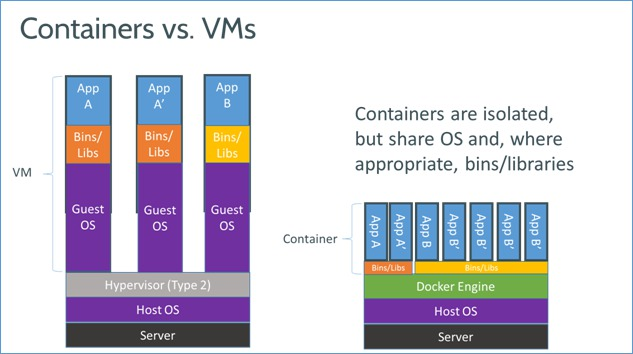
\includegraphics[scale=0.5]{img/containers_vs_vm.png}
\caption{Containers vs machines virtuelles}
\end{figure}

Les machines virtuelles possèdent leur propre OS qui embarque ses propres binaires et librairies. Ceci engendre une perte d'espace disque importante surtout si les binaires ou libraires sont communes à plusieurs machines virtuelles. De plus, démarrer une machine virtuelle prend du temps (jusqu'à plusieurs minutes). En outre, les machines virtuelles doivent installer leurs propres drivers afin de communiquer avec l'hyperviseur (logiciel s'exécutant à l'intérieur d'un OS hôte qui gère les machines virtuelles). Un avantage cependant est l'isolation complète d'une machine virtuelle qui ne peut communiquer avec les autres par défaut.

Les containers s'exécutent de manière isolée par dessus l'OS hôte qui partage ses ressources (kernel, binaires, librairies, périphériques...). Plus légers, les containers démarrent en quelques secondes seulement. Sur une machine, il est tout à fait possible de lancer de milliers de containers similaires, car l'empreinte mémoire est réduite et l'espace disque occupé est partagé si les containers sont semblables. Ceci est expliqué plus en détail à la section \ref{pres-docker-systeme-fichiers-couches}. Les containers sont isolés, mais ils peuvent aussi communiquer entre eux si on leur a explicitement donné l'autorisation.

Si le lecteur désire connaître plus de détails concernant la virtualisation, il est conseillé de lire le chapitre 3.2 du rapport "\bassangPrjSemestre" de M. Loic Bassang \cite{bassang_semestre} qui amène une bonne introduction aux différents types de virtualisation.


\section{Docker images et Docker containers}
Avec Docker, une application est encapsulée avec toutes ses dépendances et sa configuration dans une \textbf{image}. 

Pour construire cette image, on utilise un Dockerfile. Il s'agit d'un fichier qui décrit les étapes de création et de configuration nécessaires à l'obtention de l'application configurée. C'est dans ce fichier qu'on retrouve l'OS à utiliser, les dépendances à installer et toutes autres configurations utiles au bon fonctionnement de l'application à déployer. 

Typiquement un Dockerfile permettant de lancer un serveur web Nginx qui affiche un "hello world" ressemble à ceci :

\begin{bashcode}
FROM alpine  # image de départ
MAINTAINER support@tutum.co  # mainteneur du Dockerfile
RUN apk --update add nginx php-fpm && \  # installation des dépendances
    mkdir -p /var/log/nginx && \
    touch /var/log/nginx/access.log && \
    mkdir -p /tmp/nginx && \
    echo "clear_env = no" >> /etc/php/php-fpm.conf
ADD www /www  # ajout des sources de l'application
ADD nginx.conf /etc/nginx/  # ajout d'un fichier de configuration
EXPOSE 80  # ouverture du port 80
CMD php-fpm -d variables_order="EGPCS" && (tail -F /var/log/nginx/access.log &) && exec nginx -g "daemon off;" # commande à lancer au lancement du container
\end{bashcode}

Source: \url{https://github.com/tutumcloud/hello-world/blob/master/Dockerfile}

Un Dockerfile est en quelque sorte la recette de cuisine qui permet de construire une image Docker.

Une fois l'image construite, on peut exécuter l'application dans un container. Un container Docker est donc une instance de l'image fraîchement créée. La figure \ref{docker-dockerfile-image-container} montre les relations entre un Dockerfile, une image et un container.

\begin{figure}[hbtp]
\centering
\includegraphics[scale=0.7]{img/docker-dockerfile-image-container.png}
\caption{Dockerfile, image et container}
\label{docker-dockerfile-image-container}
\end{figure}


\section{Système de fichiers en couche}\label{pres-docker-systeme-fichiers-couches}
Chaque image Docker est composée d'une liste de couches (\textit{layers}) superposées en lecture seule\cite{understanding_image_container_driver_storage}. Chaque couche représente la différence du système de fichiers par rapport à la couche précédente. Sur la figure \ref{docker-image-layers}, on peut voir 4 couches (identifiables avec des ID) et leur taille respective.

\begin{figure}[hbtp]
\centering
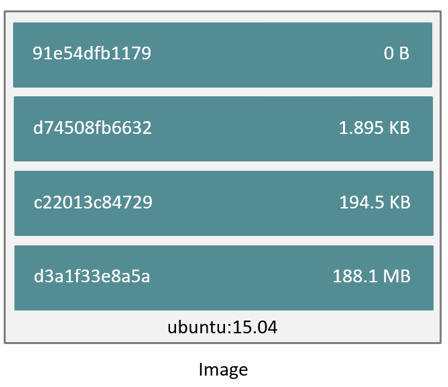
\includegraphics[scale=0.8]{img/image-layers}
\caption{Couches d'une image Docker}
\label{docker-image-layers}
\end{figure}

À la création d'un container, une nouvelle couche fine est ajoutée. Cette couche, appelée "container layer" est accessible en écriture durant l'exécution du container. La figure \ref{docker-container-layers} le montre clairement.

\begin{figure}[hbtp]
\centering
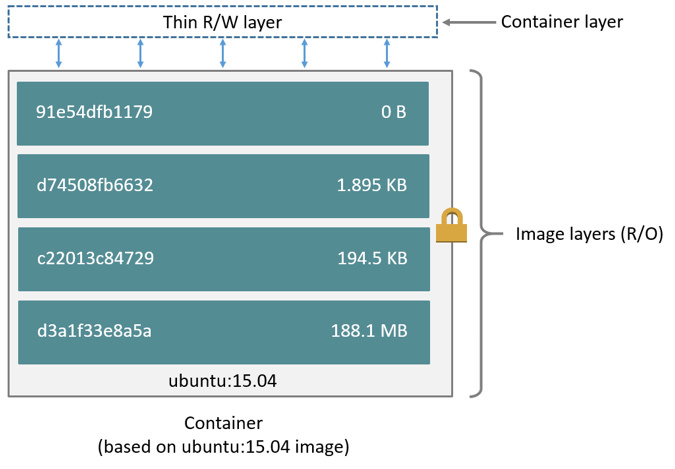
\includegraphics[scale=0.8]{img/container-layers}
\caption{Couches d'un container Docker}
\label{docker-container-layers}
\end{figure}

Un mot supplémentaire sur une nouvelle caractéristique arrivée avec Docker 1.10 (mars 2016); avant cette version, Docker attribuait des UUID\footnote{UUID : \url{https://fr.wikipedia.org/wiki/Universal_Unique_Identifier}} générés aléatoirement pour identifier les couches d'une image. Désormais, ces UUID sont remplacés par des hash appelés \textit{secure content hash}.

Les différences principales entre un UUID et un hash sont :
\begin{itemize}
\item Un UUID est généré aléatoirement, donc deux images exactement identiques auront un UUID différent alors qu'en utilisant un hash, le résultat sera identique
\item Avec les UUID, même si la probabilité est rare\footnote{Probabilité de doublon : \url{https://en.wikipedia.org/wiki/Universally_unique_identifier\#Random_UUID_probability_of_duplicates}}, il est possible de générer deux fois le même UUID ce qui peut poser des problèmes lors de la construction des images
\item Une image téléchargée chez une personne A aura un UUID différent que la même image téléchargée chez une personne B. Impossible de s'assurer de l'intégrité de l'image téléchargée en se basant sur l'UUID. En utilisant le hash, on s'assure du même résultat si l'image est identique
\end{itemize}

\vspace{2mm}
Par conséquent, Docker avance les avantages suivants:
\begin{itemize}
\item Intégrité des images téléchargées et envoyées (sur Docker Hub par exemple)
\item Évite les collisions lors de l'identification des images et des couches
\item Permet de partager des couches identiques qui proviendraient de \textit{build} différents
\end{itemize}

Le dernier point est relativement intéressant. En effet, si deux images de base (Ubuntu et Debian) sont différentes, mais qu'une couche supérieure est identique (par exemple l'ajout d'un même fichier texte) alors cette couche supérieure peut être partagée entre les deux images (puisqu'elle possède le même hash). Ceci peut potentiellement offrir un gain d'espace disque conséquent si plusieurs images partagent plusieurs couches identiques. Ceci n'aurait pas pu être possible avec les UUID, car les deux couches auraient produit deux UUID différents. Un exemple est visible à la figure \ref{shared-layer-hash}

\begin{figure}[hbtp]
\centering
\includegraphics[scale=0.7]{img/shared-layer-hash}
\caption{Couche partagée entre deux images Docker}
\label{shared-layer-hash}
\end{figure}

D'autres explications plus détaillées sur le système de fichiers en couches ont fait l'objet du chapitre 5.4.1 du rapport "\bassangPrjSemestre" de M. Loic Bassang.


\section{Isolation}\label{pres-docker-isolation}
Docker met en avant le fait que ses containers soient isolés du système hôte. Pour ce faire, Docker utilise des mécanismes fournis par le kernel. On peut citer parmi ces mécanismes les \textit{namespaces} et \textit{cgroups}.

\subsection{Les namespaces}
Les namespaces permettent d'isoler certaines fonctionnalités d'un système d'exploitation utilisant Linux. Comme chroot permet aux processus de voir comme racine un dossier isolé du système et non pas la "vraie" racine, les namespaces isolent certains aspects du système comme les processus, les interfaces réseaux, les points de montage, etc.

Jusqu'à très récemment (docker < 1.10.0), Docker supportait les namespaces suivants\cite{docker_1_10_user_namespace}:

\begin{itemize}
\item PID namespace, chaque conteneur a ses propres id de processus
\item UTS namespace, pour avoir son propre hostname
\item IPC namespace, qui permet d'isoler les Communications Inter-Processus
\item Network namespace, chaque conteneur peut avoir sa propre interface réseau, son IP, ses règles de filtrage
\end{itemize}

Docker a désormais ajouté le support d'un nouveau namespace: user namespace. Celui-ci permet à un processus d'avoir les droits root au sein d'un namespace, mais pas en dehors. Avant, Docker lançait les containers en root ce qui pouvait poser des problèmes de sécurité si un processus dans le container venait à en sortir; il se retrouverait root sur le système hôte. Avec la prise en charge de ce namespace, un container Docker a l'impression d'être root alors qu'il n'est, en réalité, qu'un utilisateur normal sur le système hôte.

\subsection{cgroups - Control Groups}
Cgroups (control groups) est une fonctionnalité du kernel pour limiter, prioriser, isoler et contrôler l'utilisation des ressources (CPU, RAM, utilisation disque, utilisation réseau...). Pour limiter les ressources, cgroups propose de créer un groupe (profil) qui décrit les limitations à respecter. Par exemple, Si on crée un groupe appelé "groupe 1" et qu'on exige de lui qu'il n'utilise qu'au maximum 25\% de la charge CPU et n'utilise qu'au maximum 100 MB de RAM. Alors, il devient possible de lancer des programmes qui appartiennent à ce groupe et qui respectent les limites fixées.

Lorsqu'on utilise la commande \code{docker run} de Docker pour lancer un container, Docker peut utiliser cgroups et ainsi limiter les ressources du container\footnote{Docker - Runtime constraints on resources: \url{https://docs.docker.com/engine/reference/run/\#runtime-constraints-on-resources}}.

\section{Contraintes liées au monde de l'embarqué}
On entend par système embarqué, un système qui est/peut être léger, autonome, à puissance limitée, à stockage réduit, avec un OS minimal et souvent connecté.

Dans le monde de l'embarqué, il existe plusieurs problèmes récurrents lorsqu'on développe, déploie et maintient une application sur une cible. On peut citer les problèmes suivants :

\begin{itemize}
\item Cross-compilation souvent obligatoire
\item Aucune interface graphique
\item Installation et configuration des dépendances sur la cible
\item Mises à jour de l'application et de ses dépendances
\item Tests et journalisation (logs)
\item Limiter l'utilisation en CPU, RAM et disque
\end{itemize}

Bien que ces problèmes peuvent être aussi présents dans le cas d'un développement desktop, ils ne sont pas aussi préoccupants.

Docker peut être utile dans le cadre d'une application embarquée, car il permet une maintenance plus aisée de l'application, car on peut \textbf{versionner son installation et sa configuration ainsi que celle de ses dépendances}. Ceci permet de plus facilement mettre à jour une application, mais également de pouvoir revenir à une version précédente. De plus, si un accès réseau est disponible, il est même possible d'administrer Docker à distance depuis un poste de développement en se connectant au \textit{deamon} Docker de la cible.

Cependant, il reste quelques freins et prérequis pour pouvoir utiliser Docker sur une carte embarquée :

\textbf{GNU/Linux : } Il faut un système GNU/Linux et si possible une distribution qui intègre Docker dans ses packages

\textbf{Images compatibles : } Les images doivent être compatibles avec la plateforme de la cible. Les images x64 ne fonctionnent pas sur ARM. Actuellement, la majorité des images sont basées sur une image de base x64. Dans la plupart des cas, il suffit de trouver l'équivalent ARM de l'image de base. Par exemple, à la lecture d'un Dockerfile, il suffit de remplacer \code{FROM ubuntu} par \code{FROM armhf/ubuntu} pour que l'image arrive à se construire. Dans les autres cas, il faudra adapter les instructions du Dockerfile.

\textbf{Espace disque limité : } Il faut veiller à l'utilisation de l'espace disque. En effet, la plupart des images se basent sur des Ubuntu (~400 MB) ou des Debian (~300 MB) ce qui peut être trop volumineux pour un système embarqué. De plus plusieurs versions de ces images peuvent être téléchargées si les Dockerfiles le spécifient. Par exemple, \code{FROM ubuntu:14.04} pour l'image 1 et \code{FROM ubuntu:15.10} pour l'image 2. On favorisera l'utilisation d'une image de base légère, comme Alpine Linux\footnote{Alpine Linux : \url{http://www.alpinelinux.org/}}, commune à plusieurs applications ou processus tournant sur la cible. 


\chapter{Matériel utilisé et mise en place de la cible}

Ce chapitre présente le matériel utilisé dans le projet ainsi que son installation et sa configuration de base.

Afin de réaliser ce projet, une carte embarquée \odroid a été mise à disposition afin d'y faire tourner Docker.

\section{La carte \odroid}

Cette carte possède les caractéristiques suivantes \cite{hardkernel_odroid_xu3}:

\begin{itemize}
\item Samsung Exynos5422 Cortex™-A15 1.8Ghz quad core and Cortex™-A7 quad core CPUs
\item Mali-T628 MP6(OpenGL ES 3.0/2.0/1.1 and OpenCL 1.1 Full profile)
\item 2Gbyte LPDDR3 RAM at 933MHz (14.9GB/s memory bandwidth) PoP stacked
\item eMMC5.0 HS400 Flash Storage
\item USB 3.0 Host x 1, USB 3.0 OTG x 1, USB 2.0 Host x 4
\item HDMI 1.4a for display
\end{itemize}

\begin{figure}[hbtp]
\centering
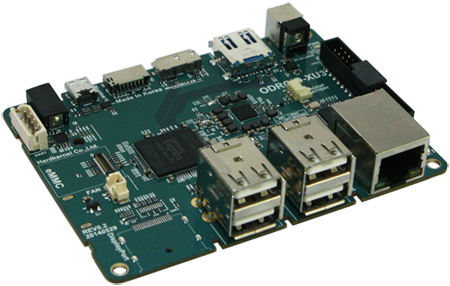
\includegraphics[scale=0.5]{img/ODROIDXU3Lite.jpg}
\caption{\odroid}
\end{figure}

Lien vers le constructeur : \url{http://www.hardkernel.com/main/products/prdt_info.php?g_code=G141351880955}.

\section{Installation du système}

Initialement, il était prévu de générer un système d'exploitation minimal qui aurait été capable de faire tourner Docker et des containers. Malheureusement, il n'a pas été possible de cross compiler Docker \textit{et son daemon} afin de lancer des containers sur ce système minimal. Plus d'informations sont disponibles dans le rapport "\oldreportname".

Ainsi, il a été décidé, de la même manière que pour le travail de bachelor précédent, d'utiliser une distribution GNU/Linux proposant Docker dans ses packages. Le choix s'est donc porté sur \textbf{Archlinux ARM} \footnote{Arch Linux ARM : \url{https://archlinuxarm.org/}}.

Sur la page wiki de la distribution (\url{https://archlinuxarm.org/platforms/armv7/samsung/odroid-xu3}), on peut suivre un guide de génération de la carte SD qui contient le système d'exploitation. Une copie de ce guide est disponible à l'appendice \ref{install_alarm_odroid}.


\section{Installation de Docker}
Une fois le système installé et démarré, il convient d'installer Docker depuis les dépôts de la distribution.

Ceci peut être accompli avec les commandes suivantes :

\begin{bashcode}
pacman -Syyu
reboot
pacman -S docker
systemctl enable docker
systemctl start docker
docker version
\end{bashcode}

Sortie:

\begin{bashcode}
Client:
 Version:      1.10.3
 API version:  1.22
 Go version:   go1.6
 Git commit:   20f81dd
 Built:        Sat Mar 12 12:49:56 2016
 OS/Arch:      linux/arm

Server:
 Version:      1.10.3
 API version:  1.22
 Go version:   go1.6
 Git commit:   20f81dd
 Built:        Sat Mar 12 12:49:56 2016
 OS/Arch:      linux/arm
 \end{bashcode}


\chapter{Objectif 3 - Docker et la sécurité}

\section{Situation actuelle}
Pour cette partie du projet, l'objectif est le suivant : Analyser et évaluer l'aspect sécurité de Docker dans le cadre d'une utilisation avec une carte embarquée.

Pour rappel, on utilise la carte \odroid. Un des objectifs de ce projet était de générer un système GNU/Linux minimal contenant un binaire Docker cross-compilé. Malheureusement, cet objectif n'a pas abouti comme expliqué dans le rapport "\oldreportname".

Pour continuer sur la partie sécurité, il a été choisi d'utiliser une distribution GNU/Linux compatible avec la carte et qui propose dans ces dépôts un package Docker précompilé. Tout comme le travail précédent de M. Loïc Bassang, Arch Linux ARM a été sélectionné.

\section{Structure de la suite du document}

Pour ce projet, il a été décidé d'étudier la question de la sécurité avec Docker avec une approche en couches. A peu à la manière du modèle OSI\footnote{Modèle OSI: \url{https://fr.wikipedia.org/wiki/Mod\%C3\%A8le_OSI}} en réseau, chaque couche représente un ensemble de fonctionnalités qui, dans le cas de ce projet, doit faire l'objet d'une évaluation de la sécurité.

L'étude de la sécurité de Docker a donc été séparée avec les couches \textit{arbitraires} suivantes:

\begin{itemize}

\item Compilation et installation de Docker : en particulier les options  de compilation

\item \nameref{config_systeme_os_hote} : configuration du kernel, configuration des options de lancement de Docker, etc.

\item \nameref{creation_utilisation_images_docker} : Bonnes pratiques et contraintes liées au monde de l'embarqué

\item \nameref{utilisation_containers} : options de lancement

\end{itemize}

\textbf{Remarque : } Chacune de ces couches fait l'objet d'un chapitre dans ce rapport excepté le premier point : Compilation et installation de Docker. En effet, celui-ci n'est pas traité car, comme annoncé précédemment, la cross compilation de Docker sur un système ARM n'a pas aboutie. L'effort est alors concentré sur les autres points.


\chapter{Configuration du système d'exploitation hôte}\label{config_systeme_os_hote}
Dans ce chapitre, on présente diverses bonnes pratiques et configurations dans le but de sécuriser Docker et/ou le système l'hébergeant.

Parmi ces techniques, on peut citer :

\begin{itemize}
\item Création d'une partition chiffrée pour stocker les données de Docker (containers et images)
\item Modification des options de lancement du \textit{daemon} Docker
\end{itemize}


\section{Passage en revue du benchmark de sécurité : CIS Docker 1.11.0 Benchmark}
Il s'agit d'un document à l'intention d'administrateurs systèmes ou spécialistes de la sécurités qui souhaitent intégrer, développer ou sécuriser des solutions qui utilisent Docker.

Le but de ce document est de proposer un éventail de recommandations concernant la sécurité de Docker sur plusieurs points. Voici les points évalués :
\begin{enumerate}
\item \textit{Host Configuration} : Recommandations pour la configuration de la machine hôte
\item \textit{Docker daemon configuration} : Recommandations concernant le comportement du \textit{daemon} Docker
\item \textit{Docker daemon configuration files} : Recommandations concernant la permission des fichiers et dossiers de configuration du \textit{daemon} Docker
\item \textit{Container Images and Build File} : Recommandations concernant les images de base et les fichiers de build
\item \textit{Container runtime} : Recommandations sur les options de lancement des containers
\item \textit{Docker Security Operations} : Rappels des bonnes pratiques concernant la sécurité de Docker
\end{enumerate}

Lien : \url{https://benchmarks.cisecurity.org/tools2/docker/CIS_Docker_1.11.0_Benchmark_v1.0.0.pdf}

Dans cette partie du rapport, quelques points de ce benchmark seront analysés et appliqués à la cible dans des conditions les plus réelles possibles.

\subsection{Situation actuelle}
Avant de chercher à sécuriser la cible, il faut connaître son état de sécurisation actuel. Pour ce faire, il suffit de lancer le script du benchmark qui va exécuter toutes les recommandations proposées et indiquer quels points sont à corriger.

Avant de commencer, il faut lancer un container en arrière plan afin de pouvoir évaluer la partie \textit{5 - Container runtime} qui évalue les containers actuellement exécutés. Pour ce faire, on choisit de lancer en tâche de fond un serveur web sur la cible.

A faire sur la cible :
\begin{bashcode}
docker run --name=my_container -d -p 8080:80 hypriot/rpi-busybox-httpd
\end{bashcode}

Lancement du benchmark :
\begin{bashcode}
git clone https://github.com/docker/docker-bench-security.git
cd docker-bench-security/
sudo sh docker-bench-security.sh
\end{bashcode}

On obtient la sortie suivante :

\inputminted[xleftmargin=20pt, linenos=true, breaklines=true, frame=single, framesep=6pt, tabsize=2, fontfamily=courier, fontsize=\small]{text}{../../docker_security_benchmark/vanilla.log}


Comme on peut le voir, il y a plusieurs points qui sont en \textit{WARN}. Pour la suite du document, plusieurs de ces points vont être analysés et mitigés.


\subsection{1.1  - Create a separate partition for containers}
On recommande pour ce point de créer une partition séparée pour les containers. Ce point est traité à la section \ref{partition_chiffree}. Dans cette section, une étape supplémentaire est proposée; la partition est chiffrée.


\subsection{2.1  - Restrict network traffic between containers}
Par défaut, le trafic réseau est autorisé entre containers du même hôte. On devrait désactiver ce comportement par défaut et explicitement autoriser une communication entre containers grâce au "linking".

Pour remédier à ceci, il faut lancer le \textit{daemon} Docker avec cette option: \code{docker daemon --icc=false}

A faire sur la cible:

\begin{bashcode}
sudo vim /usr/lib/systemd/system/docker.service
\end{bashcode}

Ajouter l'option icc=false à l'instruction ExecStart. Le résultat devrait ressembler à ceci:

\begin{bashcode}
ExecStart=/usr/bin/docker daemon -H fd:// --icc=false
\end{bashcode}

Redémarrage du daemon:

\begin{bashcode}
sudo systemctl daemon-reload # recharge la configuration des services
sudo systemctl restart docker # relance le service docker
\end{bashcode}

Résultat du benchmark après cette modification: \code{[PASS] 2.1 - Restrict network traffic between containers}.

\subsection{2.5 - Do not use the aufs storage driver}
Pour stocker les images et les différentes couches qui les composent, Docker utilise un driver de stockage\cite{understanding_image_container_driver_storage}, \cite{docker_select_a_driver}, \cite{jpetazzoni_device_driver}. Un driver de stockage (\textit{driver storage}) est l'implémentation d'une abstraction de services liés à la gestion des couches des images et de la couche inscriptible (\textit{writable}) des containers. L'utilisation d'un driver ou d'un autre est transparent pour l'utilisateur. Cependant, une certaine implémentation, aufs, est considérée peu stable et peut causer des crashes au niveau du kernel, voir \cite{cis_benchmark} page 45. Ce driver est donc à remplacer par un autre driver de stockage comme devicemapper par exemple.

Inconvénient: aufs est le seul driver de stockage qui permet aux containers de partager la mémoire des librairies partagées. Cela peut être utile si la cible fait tourner des milliers de containers utilisant les mêmes programmes ou librairies \cite{cis_benchmark}.

Dans le cadre d'une carte embarquée, on ne va pas faire tourner des milliers de containers en même temps et par conséquent changer de driver storage n'est pas un problème.

Par défaut Docker utilise devicemapper mais suivant la distribution ou la plateforme utilisée, un autre storage driver est utilisé. Dans le cas présent, aufs est malheureusement utilisé.

Vérification que device-mapper est présent sur le système:

\begin{bashcode}
[alarm@alarm docker-bench-security]# pacman -Qi device-mapper
Name            : device-mapper
Version         : 2.02.149-1
Description     : Device mapper userspace library and tools
Architecture    : armv7h
URL             : http://sourceware.org/dm/
Licenses        : GPL2  LGPL2.1
Groups          : base
Provides        : None
Depends On      : glibc  systemd
Optional Deps   : None
Required By     : cryptsetup  docker  lvm2
Optional For    : None
Conflicts With  : None
Replaces        : None
Installed Size  : 871.00 KiB
Packager        : Arch Linux ARM Build System <builder+xu2@archlinuxarm.org>
Build Date      : Sun Apr 17 12:52:54 2016
Install Date    : Mon Apr 18 14:12:44 2016
Install Reason  : Explicitly installed
Install Script  : No
Validated By    : SHA-256 Sum
\end{bashcode}

Comme avant, on change les paramètres de lancement du \textit{daemon} Docker:

\begin{bashcode}
sudo vim /usr/lib/systemd/system/docker.service
\end{bashcode}

Ajouter l'option \code{--storage-driver=devicemapper} à l'instruction ExecStart. Le résultat devrait ressembler à ceci:

\begin{bashcode}
ExecStart=/usr/bin/docker daemon -H fd:// --icc=false --storage-driver=devicemapper
\end{bashcode}

\begin{bashcode}
sudo systemctl daemon-reload # recharge la configuration des services
sudo systemctl restart docker # relance le service docker
\end{bashcode}


\subsection{2.8 - Enable user namespace support}
Les namespaces permettent d'isoler certaines fonctionnalités d'un système d'exploitation utilisant Linux. Comme chroot permet aux processus de voir comme racine un dossier isolé du système et non pas la "vraie" racine, les namespaces isolent certains aspects du système comme les processus, les interfaces réseaux, les points de montage, etc.

Jusqu'à très récemment (docker < 1.10.0), Docker supportait les namespaces suivants:
\begin{itemize}
\item PID namespace, chaque conteneur a ses propres id de processus
\item UTS namespace, pour avoir son propre hostname
\item IPC namespace, qui permet d'isoler les Communications Inter-Processus
\item Network namespace, chaque conteneur peux avoir sa propre interface réseau, son ip, ses règles de filtrage
\end{itemize}

Pour plus de détails, voir section \ref{pres-docker-isolation}.

Il y a peu de temps, Docker ajouté le support d'un nouveau namespace\cite{docker_1_10_user_namespace}: user namespace. Celui-ci permet à un processus d'avoir les droits root au sein d'un namespace mais pas en dehors. Avant, Docker lançait les containers en root ce qui pouvait poser des problèmes de sécurité si un processus dans le container venait à en sortir; il se retrouverait root sur le système hôte. Avec la prise en charge de ce namespace, un container Docker a l'impression d'être root alors qu'il n'est, en réalité, qu'un utilisateur normal sur le système hôte.

Pour mettre en place ce mécanisme, il faut réaliser les opérations suivantes :

\begin{bashcode}
touch /etc/subuid /etc/subgid
\end{bashcode}

Et ajouter l'option \code{--userns-remap=default} au démarrage du \textit{daemon} Docker.

Malheureusement, il a été impossible de démarrer le \textit{daemon} avec cette option que ce soit sur la cible (Archlinux, kernel 3.10.96), sur un portable Archlinux (kernel 4.5.4) ou sur un autre portable Xubuntu 16.04 (kernel 4.4.0). Le \textit{daemon} refusait de démarrer ou se bloquait. Il semblerait que cela ne soit pas un cas isolé. En effet plusieurs issues (\#20751, \#21130\footnote{Docker issues : \url{https://github.com/docker/docker/issues}}) ont été ouvertes sur le \textit{repository} Github de Docker.


\subsection{2.11 - Use authorization plugin}
Le modèle de permission Docker par défaut est tout ou rien. Tout utilisateur qui a accès au \textit{daemon} Docker peut effectuer n'importe quelles opérations sur tous les containers. Dans le cas où l'on a besoin d'un contrôle plus fin, il est possible de créer des plugins d'autorisation (\textit{authorization plugins}) et les ajouter à la configuration du \textit{daemon} Docker. Il est, par exemple, possible de définir que l'utilisateur Bob ne puisse pas arrêter les containers mais uniquement les lister.

Un plugin d'autorisation approuve ou refuse les requêtes du client (un utilisateur)  vers le \textit{daemon} en se basant sur le contexte actuel d'authentification et le contexte de commande. Le contexte d'authentification contient toutes les détails de l'utilisateur et de la méthode d'authentification et le contexte de commande contient toutes les données utiles à la requête de l'utilisateur.

\textbf{Remarque : } La communication entre le \textit{daemon} et le client\cite{docker_doc_daemon} se fait à travers un socket Unix (\code{/var/run/docker.sock}) mais peut aussi se faire via un socket TCP (\code{tcp://0.0.0.0:2375}) pour accéder au \textit{daemon} de manière distante. Grâce à ce mécanisme, Docker propose \textit{Docker Remote API}\cite{docker_doc_remote_api} une API \textit{REST-like} qui permet d'accéder à la liste des containers, des images, de créer des containers, etc.

Pour créer un plugin d'autorisation, il faut respecter le contrat décrit par la \textit{Docker Plugin API}. De manière similaire à la \textit{Docker Remote API}, cette API définit un cadre afin d'étendre les possibilités de Docker comme par exemple autoriser ou refuser l'accès à certaines fonctionnalités de Docker pour un utilisateur ou un groupe donné.


Maintenant les notions de communication client \textit{daemon} et API REST éclaircies, on peut enfin voir l'architecture de base des plugins d'autorisation.

\begin{figure}[H]
    \subfloat[Cas où la requête est autorisée]{%
      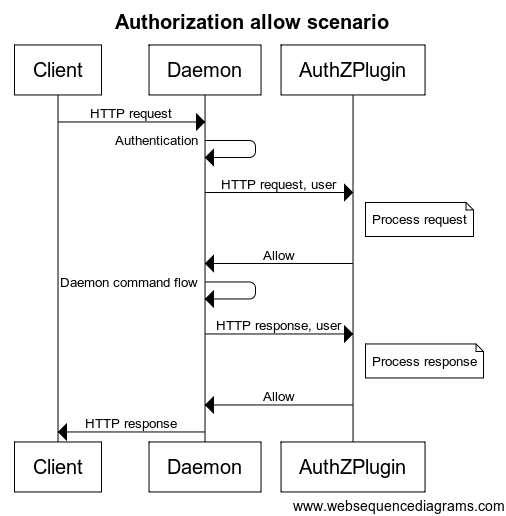
\includegraphics[width=0.45\textwidth]{img/auth_plugins/authz_allow.png}
    }
    \hfill
    \subfloat[Cas où la requête est refusée]{%
      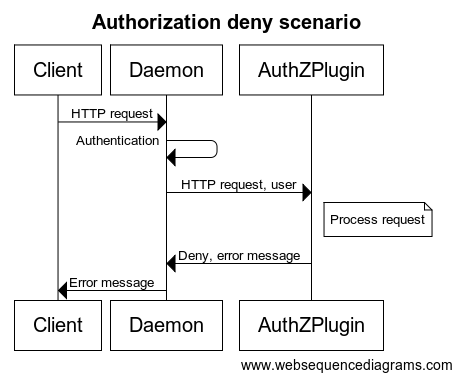
\includegraphics[width=0.45\textwidth]{img/auth_plugins/authz_deny.png}
    }

    \caption[]{Scénarios d'autorisation Docker\protect{\footnotemark}}
\end{figure}

\footnotetext{Source des images : \url{https://docs.docker.com/engine/extend/plugins_authorization/}}

Comme on peut le voir sur les figures ci-dessus, les requêtes sont des requêtes HTTP JSON comme on peut le trouver fréquemment dans avec les API REST.

Il est possible d'utiliser plusieurs plugins en même temps. Dans ce cas, pour qu'une requête soit acceptée, il faut qu'elle puisse traverser tous les plugins (donc être approuvée par tous les plugins). Si un seul plugin refuse la requête alors elle est refusée.

La création et mise en place de plugin n'est pas présenté dans ce rapport. Néanmoins, voici un exemple de plugin : \url{https://github.com/twistlock/authz}.

\textbf{Analyse : } Dans le cas d'une utilisation embarquée, il n'est pas indispensable d'avoir recours à un contrôle plus fin de l'utilisation de Docker car :
\begin{itemize}
\item la cible est souvent mono-utilisateur
\item les containers appartiennent tous au même utilisateur. Dans le cas d'une plateforme offrant un service de type CaaS (Containers as a Service), on peut comprendre que chaque utilisateur n'ait accès qu'aux containers qu'il lance.
\end{itemize}
Par conséquent, on décide de ne pas mettre en place ce mécanisme. On rappelle que ce benchmark a surtout pour but de montrer un ensemble de bonnes pratiques et de rendre attentif à certains aspects de la sécurité avec Docker. Il n'est néanmoins pas toujours indispensable d'appliquer toutes les mesures de sécurités si on en exprime pas le besoin.


\subsection{2.12 - Configure centralized and remote logging}
Docker supporte plusieurs \textit{log drivers} (manière de journaliser). Par défaut, les logs des containers sont produits dans des fichiers JSON sur la machine hôte. Mais il est recommandé de centraliser les logs sur une machine distante pour voir et traiter les logs globalement.

Le benchmark CIS recommande d'externaliser les logs en optant pour le log driver \textit{syslog}. \textit{Syslog}\cite{developpez_syslog}\cite{wiki_syslog} est un protocole définissant un service de journaux d'évènements d'un système informatique. Son but est de transporter par réseau les messages de journalisation générés par une application (dans ce cas Docker) vers un serveur hébergeant un serveur \textit{Syslog}. Le but étant de regrouper tous les journaux au même endroit.

Pour la suite, on va mettre en place un petit exemple de démonstration qui n'a absolument pas la prétention d'être exhaustif ni sécurisé. Cet exemple a uniquement pour but de montrer un cas simple de \textit{remote logging}.

Pour cet exemple, il y a à disposition un ordinateur portable qui fait office de serveur \textit{Syslog} et la cible Odroid qui va lancer un container dont les logs sont envoyés à l'ordinateur portable. On peut voir cette configuration ci-dessous.

\begin{figure}[H]
\centering
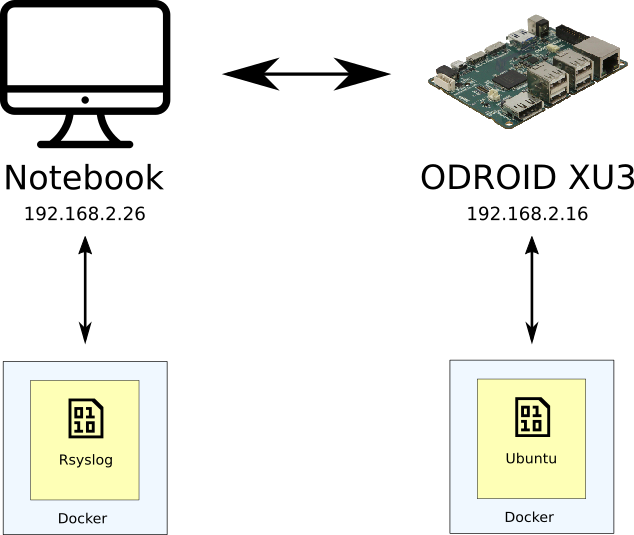
\includegraphics[scale=0.7]{img/docker_syslog.png}
\caption{Structure de démonstration Syslog}
\end{figure}

Le container (ici Ubuntu) va être lancé en indiquant que les logs doivent être envoyés au PC portable disposant d'un serveur syslog dans un container appelé rsyslog.

Pour le serveur \textit{Syslog}, un container Docker prêt à l'emploi va être utilisé. Ce container utilise une image Rsyslog dont la source se trouve ici: \url{https://hub.docker.com/r/panoptix/rsyslog/}.

Lancement du container Rsyslog sur le portable et affichage des logs distants :
\begin{bashcode}
# démarrage du container
docker run --name rsyslog -t -d -p 514:514/udp -p 514:514 panoptix/rsyslog

# affichage des logs en temps réel
docker exec -it rsyslog bash
tail -f /var/log/syslog
\end{bashcode}

Lancement du container Ubuntu (producteur de logs) sur la cible :
\begin{bashcode}
docker run -d --log-driver=syslog --log-opt syslog-address=tcp://192.168.2.26 --log-opt tag="remote" armhf/ubuntu echo "hello from Odroid"
\end{bashcode}

Ce container va lancer la commande \code{echo} et se stopper immédiatement après. Évidemment dans un cas réel, le container effectuera des opérations plus longues et produirait un plus grande quantité de logs mais ici le but est de voir le principe général.

Sur l'ordinateur portable, on peut observer l'affichage suivant :
\begin{bashcode}
May 22 18:23:42 fc6dca22947a rsyslogd: [origin software="rsyslogd" swVersion="8.11.0" x-pid="1" x-info="http://www.rsyslog.com"] start
May 22 18:38:09 192.168.2.16 docker/remote[284]: hello from Odroid
\end{bashcode}

Comme on peut le voir, on est capable de récupérer les logs de la cible sur l'ordinateur portable.

\textbf{Remarque : } Pour cet exemple, les options de logging ont été précisés au niveau du lancement du container (\code{--log-driver=XXX --log-opt syslog-address=tcp://aaa.bbb.ccc.ddd --log-opt YYY}). Idéalement, il faudrait définir par défaut toutes ces options au démarrage du \textit{daemon}. Pour ce faire, il suffit de modifier la configuration de lancement du \textit{daemon} comme il a été montré aux sections précédentes. Par exemple, on pourrait configurer le \textit{daemon} ainsi :

\begin{bashcode}
ExecStart=/usr/bin/docker daemon -H fd:// --icc=false --storage-driver=devicemapper --log-driver=XXX --log-opt syslog-address=tcp://aaa.bbb.ccc.ddd --log-opt YYY
\end{bashcode}

\textbf{Analyse : } On l'a vu les containers produisent des logs qu'il est recommandé de centraliser sur une machine distante. Pour ce faire, Docker propose plusieurs \textit{log drivers} qui permettent ce besoin. Dans cet exemple, \textit{Syslog} a été utilisé mais il existe d'autres \textit{log drivers}\footnote{Docker log drivers : \url{https://docs.docker.com/engine/admin/logging/overview/}}.

L'exemple présenté est sommaire mais il montre le principe général. Dans un cas plus pratique, par exemple un ensemble de cibles qui transmettent la température ambiante à un serveur (ou autre application IoT), on configurerait les cibles pour émettre leurs logs sur un serveur distant. Ce serveur disposerait ensuite d'une interface web affichant l'ensemble des logs des cibles et il serait ainsi possible de suivre le fonctionnement de toutes les cibles. De plus, dans un cas pratique, il faudrait aussi veiller à regarder le contenu de l'image rsyslog téléchargée et vérifier qu'elle fasse bien uniquement ce qu'on lui demande et rien de plus ou alors créer une image rsyslog de toutes pièces.


\subsection{2.13 - Disable operations on legacy registry (v1)}
Un \textit{registry} est un service responsable de l'hébergement et de la distribution d'images Docker. C'est une sorte d'App Store pour image Docker. Le \textit{registry} par défaut est Docker Hub\footnote{Docker Hub : \url{http://hub.docker.com/}}. Il est également possible d'utiliser son propre \textit{registry}. Dans tous les cas, il est recommandé de ne plus utiliser la version 1 de l'API de communication avec les \textit{registries} car la version 2 permet notamment le transfert sécurisé de données en utilisant TLS\cite{blog_docker_registry_v2}.

Pour forcer Docker a n'utiliser que des \textit{registries} v2, il suffit d'ajouter l'option \code{--disable-legacy-registry} au démarrage du \textit{daemon} Docker.

A faire sur la cible:

\begin{bashcode}
sudo vim /usr/lib/systemd/system/docker.service
\end{bashcode}

Ajouter l'option icc=false à l'instruction ExecStart. Le résultat devrait ressembler à ceci:

\begin{bashcode}
ExecStart=/usr/bin/docker daemon -H fd:// --icc=false --storage-driver=devicemapper --disable-legacy-registry
\end{bashcode}

Redémarrage du daemon:

\begin{bashcode}
sudo systemctl daemon-reload # recharge la configuration des services
sudo systemctl restart docker # relance le service docker
\end{bashcode}

Résultat du benchmark après cette modification: \code{[PASS] 2.13 - Disable operations on legacy registry (v1)}.


\subsection{4.1  - Create a user for the container}
Par défaut, lorsqu'on lance un container, l'utilisateur à l'intérieur de ce container est root. Pour des raisons évidentes de sécurité, root n'est pas toujours l'utilisateur le plus adapté quand on lance un container. De plus, si par une quelconque raison, on arrive à sortir du container, on se retrouve root sur la machine hôte !

Pour mitiger ces effets, il est possible de :
\begin{itemize}
\item Créer un utilisateur avec des droits limités dans l'image du container (\code{USER toto} dans le Dockerfile)
\item Spécifier l'utilisateur à utiliser lors du lancement du container (\code{docker run --user toto})
\item Faire croire au container qu'il est root alors qu'en réalité il s'agit d'un utilisateur à droits limités (user namespace)
\end{itemize}

La suite a pour but de montrer les différentes techniques pour changer l'utilisateur au sein du container.

\subsubsection{État initial}
On utilise l'image Alpine sans modifications et on observe les résultats suivants :

\begin{textcode}
docker run -it alpine /bin/sh
/ # whoami
root
/ # touch /root.txt
/ # ls /root.txt
/root.txt
/ # ls -l /root.txt
-rw-r--r--    1 root     root             0 May 23 13:41 /root.txt
\end{textcode}

On voit que par défaut l'utilisateur dans le container est root. Cet utilisateur peut donc écrire un fichier à la racine.

\subsubsection{Dans le Dockerfile}
Pour l'exemple qui suit, on va créer une image qui utilise Alpine Linux comme base. Cette image est modifiée pour qu'elle se lance par défaut avec un utilisateur toto qui a des droits limités.

\begin{bashcode}
mkdir alpine-user
vim Dockerfile
\end{bashcode}

Dans le Dockerfile, on écrit :
\begin{bashcode}
FROM alpine

# tâches nécessitant un accès root
# par exemple, installer des packages
RUN apk update && apk add vim

# fin des tâches demandant un accès root
# passage à un user à droits limités
RUN adduser -h /home/toto -s /bin/sh -D toto
USER toto

CMD ["/bin/sh"]
\end{bashcode}

On utilise donc l'image de base d'Alpine sur laquelle on effectue des tâches administratives nécessitant root. Une fois ces tâches effectuées, il n'est plus nécessaire d'être root. On crée alors un utilisateur à droit limité appelé toto. C'est cet utilisateur qui sera utilisé par défaut au lancement d'un container utilisant cette image.

\begin{textcode}
docker run -it alpine-user
/ whoami
toto
/ touch /toto.txt
touch: /toto.txt: Permission denied
\end{textcode}

Ici, on voit que l'utilisateur en cours est toto et qu'il n'a pas les droits root.

\subsubsection{Au lancement du container}
Il est également possible de spécifier l'utilisateur à utiliser au lancement du container grâce à l'option \code{--user}.

Les cas suivants sont testés :
\begin{itemize}
\item root : on peut spécifier root si l'image a défini un autre utilisateur par défaut. Utilisation déconseillée.
\item nobody : l'utilisateur nobody est un utilisateur aux droits très limités et la plupart des distributions l'intègre de base donc pas besoin le créer expressément.
\item gary : cas où l'utilisateur existe sur l'hôte mais pas dans le container
\item toto : cas où l'utilisateur n'existe pas sur l'hôte mais dans le container
\end{itemize}

\textbf{Utilisateur root} :
\begin{textcode}
> docker run --user root -it alpine-user
/ # whoami
root
/ # touch /root.txt
/ # ls -al /root.txt
-rw-r--r--    1 root     root             0 May 23 19:35 /root.txt
\end{textcode}

Le container est lancé en root. On peut écrire à la racine sans souci.

\textbf{Utilisateur root} :
\begin{textcode}
> \$ docker run --user nobody -it alpine-user
~ \$ whoami
nobody
~ \$ touch /nobody.txt
touch: /nobody.txt: Permission denied

\end{textcode}

Le container est lancé avec l'utilisateur nobody (présent sur l'OS hôte et surtout dans le container). L'écriture sur \code{/} est refusée.


\textbf{Utilisateur gary} :
\begin{textcode}
> docker run --user gary -it alpine-user
docker: Error response from daemon: linux spec user: Unable to find user gary.
\end{textcode}

Lancer un container avec un utilisateur qui n'existe pas dans le container n'est pas possible.

\textbf{Utilisateur toto} :
\begin{textcode}
> \$ docker run --user toto -it alpine-user
/ \$ whoami
toto
/ \$ touch /toto.txt
touch: /toto.txt: Permission denied
\end{textcode}

Le container est lancé avec l'utilisateur toto (absent sur l'OS hôte et mais présent dans le container). L'écriture sur \code{/} est refusée.

\subsubsection{Analyse}
On remarque que par défaut, les containers sont lancés en root. Si le container n'a pas besoin d'avoir des accès root, il est fortement recommandé de construire une image mettant en place un utilisateur à droits limités. Dans le cas où l'on utilise une image écrite par quelqu'un d'autre, on peut essayer de lancer avec l'utilisateur nobody si on estime qu'elle n'a pas besoin des droits root pour fonctionner. Évidemment, cela ne fonctionnera pas si l'image a réellement besoin des droits root comme par exemple pour installer des packages.

Le dernier cas concerne l'utilisation du user namespace. Ici c'est différent, on mappe un utilisateur standard de la machine hôte à l'utilisateur root du container. Ainsi, on peut effectuer des tâches nécessitant les droits root dans le container. Cependant, si le processus au sein du container vient à s'en échapper, il n'est pas root mais l'utilisateur mappé aux droits limités.


\subsection{4.5  - Enable Content trust for Docker}
\textbf{Rappel :} Un \textit{registry} (Docker Hub par exemple) héberge des \textit{repositories} et un \textit{repository} contient plusieurs images. Chacune de ses images est une "couche" de l'application ou du processus proposé(e) par un utilisateur.

Docker Content Trust\cite{blog_docker_content_trust}\cite{mouat_2005} est une fonctionnalité de Docker arrivée avec la version 1.8 qui permet de vérifier les auteurs des images Docker. Avant qu'un auteur publie une image sur un \textit{registry} distant (par exemple Docker Hub), Docker Engine signe l'image en local avec la clé privée de l'auteur. Quand l'image est rapatriée (\textit{pulled}), Docker Engine compare la clé publique contenue dans le certificat qui accompagne l'image avec la clé publique de l'auteur pour vérifier que l'image téléchargée n'a pas été altérée et est à jour.

Docker Content Trust n'est pas activé par défaut. Une fois activé, ces mécanismes de vérifications et de contrôles sont transparents pour l'utilisateur Docker. Les commandes \code{docker pull}, \code{docker push}, \code{docker build}, \code{docker create} et \code{docker run} sont utilisées de la même façon à la différence qu'elles opèrent sur du contenu signé.

Voici dans les grandes lignes comment fonctionne ce système :

\begin{figure}[H]
\centering
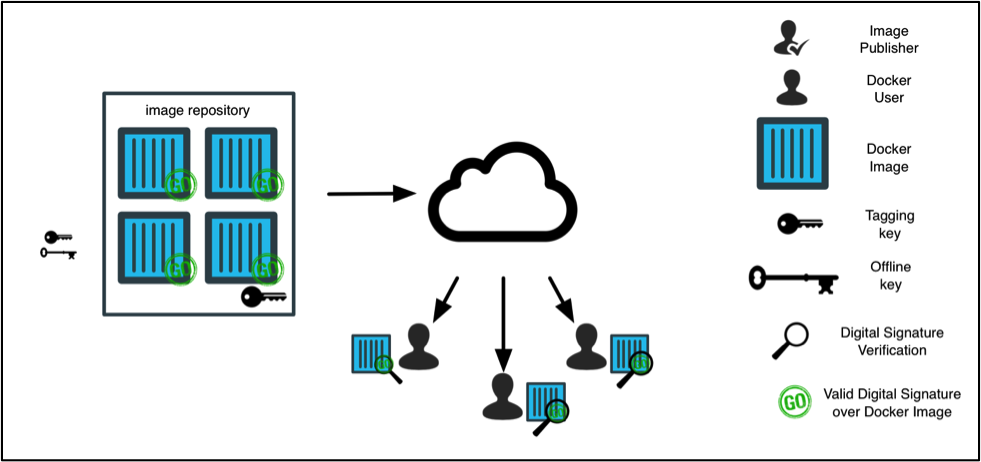
\includegraphics[scale=1]{img/dct1.png}
\caption{Vue d'ensemble de Docker Content Trust}
\end{figure}

Soient deux utilisateurs Docker, Alice et Bob. Alice est une utilisatrice qui met à disposition des images dans un \textit{repository} sur un \textit{registry} (Docker Hub, par exemple). Bob est un utilisateur qui veut télécharger (comprendre \textit{pull}) les images qu'Alice a mises à disposition.

Quand Alice désire publier une image dans un de ses \textit{repositories} appelé AliceSoft, deux clés sont générées, la \textit{Tagging Key} et la \textit{Offline Key}. Ces deux clés sont détaillées plus bas. Les images sont signées en utilisant la \textit{Tagging Key} qui est signée avec la \textit{Offline Key}.

Bob désire ensuite télécharger cette image. Comme c'est la première fois que Bob télécharge une image du \textit{repository} AliceSoft, Docker Engine va télécharger en HTTPS le certificat de ce \textit{repository}. Les fois suivantes, on réutilise le certificat téléchargé. Puis, Docker Engine compare la clé contenue dans le certificat avec la clé de l'image téléchargée.

Docker Content Trust utilise deux clés distinctes, une \textit{Offline Key} et une \textit{Tagging Key} qui sont générées la première fois qu'un auteur pousse une image. Elles sont stockés côté client (chez Alice dans l'exemple). Chacun de ses \textit{repositories} possède une \textit{Tagging Key} unique. La première fois que Bob veut télécharger une image d'Alice, il établit une confiance avec le \textit{repository} d'Alice en utilisant la \textit{Offline Key}.

\begin{itemize}
\item \textbf{La Tagging Key} : est générée pour chaque nouveau \textit{repository} qu'un auteur possède. Elles peuvent être exportées et partagées avec toute personne ou système qui exprime le besoin de signer du contenu (typiquement une image) dans ce \textit{repository}, par exemple, un \textit{repository} appartenant à un groupe de personnes.
\item \textbf{La Offline Key} : est la clé la plus importante car c'est elle qui permet d'établir la confiance pour le \textit{repository} ou les \textit{repositories} qu'elle contrôle. Cette clé est aussi utilisée pour effectuer des rotations sur les autres clés existantes (si une clé a été compromise par exemple). La \textit{Offline Key} est secrète, doit être stockée dans un endroit sûr et doit également être sauvegardée.
\end{itemize}


pourquoi on le change

Grâce à ces protections, Docker annonce une meilleure sécurité quant à la provenance des images téléchargées. On évite ainsi plusieurs types d'attaque comme :
\begin{itemize}
\item Man In the Middle (l'attaquant se place entre le \textit{registry} et l'utilisateur et altère l'image téléchargée)
\item Les attaques par rejeu (un attaquant force l'utilisateur à télécharger une image valide mais ancienne dont il sait qu'elle contient des vulnérabilités connues)
\item Les clés compromises (l'attaquant à volé la clé ou l'a cassée)
\end{itemize}

Ces garanties sont justifiées sur le blog de Docker à l'adresse suivante : \url{https://blog.docker.com/2015/08/content-trust-docker-1-8/}.

\subsubsection{Mise en place}
Pour activer Docker Content Trust, il suffit de définir la variable d'environnement \linebreak \code{export DOCKER\_CONTENT\_TRUST=1}. Définir une variable d'environnement dans un terminal est valable durant la durée de la session et pour l'utilisateur courant. Pour définir cette variable de manière permanente et pour tous les utilisateurs, il peut modifier le fichier \code{/etc/environment} et ajouter la variable d'environnement voulue.

\begin{bashcode}
sudo vim /etc/environment
\end{bashcode}

Et ajouter :
\begin{bashcode}
#
# This file is parsed by pam_env module
#
# Syntax: simple "KEY=VAL" pairs on separate lines
#
DOCKER_CONTENT_TRUST=1
\end{bashcode}

Après avoir redémarré, on relance le benchmark et on obtient la sortie suivante : \code{[PASS] 4.5  - Enable Content trust for Docker}

\subsubsection{Utilisation dans la pratique}
Désormais, tous les \code{docker pull} que l'on fait exige que les images téléchargées soient signées. 

Il existe donc 3 cas :
\begin{enumerate}
\item L'image n'est pas signée et fait une erreur
\item L'image n'est pas signée mais on veut quand même la télécharger
\item L'image est signée
\end{enumerate}

Voici les 3 cas en pratique :

\textbf{1. Image non-signée :}
\begin{textcode}
> docker pull armv7/armhf-debian
Using default tag: latest
Error: remote trust data does not exist for docker.io/armv7/armhf-debian: notary.docker.io does not have trust data for docker.io/armv7/armhf-debian
\end{textcode}

Quand on essaie de \textit{pull} une image (mais c'est également le cas pour d'autres commandes comme \code{docker run}) et que celle-ci n'est pas signée, alors Docker indique qu'il n'a pas pu établir une confiance avec cette image.

Ici, il existe deux choix : soit on ignore ce message et on télécharge tout de même cette image, soit on cherche une autre image similaire qui a été signée.

\textbf{2. Image non-signée, avertissement ignoré :}

Pour quand même télécharger cette image, on peut utiliser le flag \code{--disable-content-trust} sur les commandes Docker concernées ou alors on peut redéfinir la variable d'environnement \code{DOCKER\_CONTENT\_TRUST} à 0.

\begin{textcode}
> docker pull --disable-content-trust armv7/armhf-debian
Using default tag: latest
latest: Pulling from armv7/armhf-debian
cc738ad9b216: Pull complete 
a3ed95caeb02: Pull complete 
Digest: sha256:7c04a67927a012551a19d359f745480ae77afed229eb1ab0eac403b45fbf5f37
Status: Downloaded newer image for armv7/armhf-debian:latest
\end{textcode}

On note que pour lancer un container, il faut repréciser le flag sans quoi le container refusera de se lancer.

\begin{textcode}
> docker run -it armv7/armhf-debian
docker: notary.docker.io does not have trust data for docker.io/armv7/armhf-debian.
See 'docker run --help'.
\end{textcode}

\begin{textcode}
> docker run --disable-content-trust -it armv7/armhf-debian
root@28f7dca7a5f5:/# 
\end{textcode}

\textbf{3. Image signée}
Dans la pratique on se rend compte qu'il n'y a pas encore beaucoup d'images compatible ARM qui sont signées. D'ailleurs pour cet exemple, on \code{pull} une image signée x64 sur la cible. Il est évident que cette image ne va pas pouvoir être lancée mais c'est juste pour l'exemple.

\begin{textcode}
> docker pull ubuntu
Using default tag: latest
Pull (1 of 1): ubuntu:latest@sha256:1bea66e185d[...]
sha256:1bea66e185d[...]: Pulling from library/ubuntu
203137e8afd5: Pull complete 
2ff1bbbe9310: Pull complete 
933ae2486129: Pull complete 
a3ed95caeb02: Pull complete 
Digest: sha256:1bea66e185d[...]
Status: Downloaded newer image for ubuntu@sha256:1bea66e185d[...]
Tagging ubuntu@sha256:1bea66e185d[...] as ubuntu:latest
\end{textcode}

Heureusement, il existe un moyen de garantir que l'intégrité de l'image même si celle-ci n'a pas été signée. La seule condition est qu'il faut connaître le \textit{digest} (empreinte) de l'image.

\begin{textcode}
> docker pull armhf/alpine@sha256:9f7b4923[...]
sha256:9f7b4923[...]: Pulling from armhf/alpine
06da76670c3f: Pull complete 
Digest: sha256:9f7b4923[...]
Status: Downloaded newer image for armhf/alpine@sha256:9f7b4923[...]
\end{textcode}

Ici par exemple, on remarque que l'image \code{armhf/alpine:latest} n'est pas signée. Par contre, si on spécifie le \textit{digest} de cette image, il est possible de la téléchargée sans avoir besoin d'indiquer le flag \code{--disable-content-trust}.

De plus, indiquer le \textit{digest} dans le Dockerfile pour la commande \code{FROM xxx} est une bonne pratique car on s'assure de toujours avoir la même image qui est téléchargée et de ne pas avoir de surprise si l'image a été mise à jour.

On peut trouver ce \textit{digest} quand on pull une image :
\begin{textcode}
Digest: sha256:9f7b4923[...]
\end{textcode}

Ou avec la commande \code{docker images --no-trunc} :

\begin{textcode}
> docker images --no-trunc
REPOSITORY          TAG     IMAGE ID           CREATED        SIZE
armhf/alpine        <none>  sha256:a9e1[...]   14 hours ago   3.906 MB
ubuntu              latest  sha256:9743[...]   9 weeks ago    187.9 MB
ubuntu              <none>  sha256:9743[...]   9 weeks ago    187.9 MB
armv7/armhf-ubuntu  latest  sha256:43b1[...]   7 months ago   130.5 MB
armv7/armhf-debian  latest  sha256:8d68[...]   8 months ago   104.9 MB
\end{textcode}

\subsection{5.3  - Restrict Linux Kernel Capabilities within containers}\label{ss-restrict-kernel-capa}
Les containers sont lancés avec des permissions (\textit{kernel capabilities}) par défaut. Ces permissions permettent d'effectuer des opérations qui demandent les droits root. Par exemple. la permission \code{net\_bind\_service} permet à un container de \textit{binder} un port privilégié (ports inférieurs à 1024). Il est possible et recommandé de ne donner que les permissions qui sont strictement nécessaire à l'exécution du container. L'idée ici étant de ne donner aux containers qu'une partie des droits root, voire carrément aucun.

Il est par exemple inutile pour la plupart des containers d'avoir la permission \code{SYS\_MODULE} qui permet charger et de décharger des modules kernel.

Les permissions accordées par défaut sont les suivantes\cite{github_docker_kernel_capabilities} :
\begin{itemize}
\item CAP\_CHOWN
\item CAP\_DAC\_OVERRIDE
\item CAP\_FSETID
\item CAP\_FOWNER
\item CAP\_MKNOD
\item CAP\_NET\_RAW
\item CAP\_SETGID
\item CAP\_SETUID
\item CAP\_SETFCAP
\item CAP\_SETPCAP
\item CAP\_NET\_BIND\_SERVICE
\item CAP\_SYS\_CHROOT
\item CAP\_KILL
\item CAP\_AUDIT\_WRITE
\end{itemize}

La liste complète des permissions et leur description se trouve ici : \url{http://man7.org/linux/man-pages/man7/capabilities.7.html}

Pour ajouter ou supprimer des permissions, on utilise les arguments \code{--cap-add} et \code{--cap-drop} de la commande \code{docker run}.

Voici un exemple. Ici on veut montrer ce qui se passe quand on retire la permission d'effectuer un \code{chroot}.
\begin{textcode}
> docker run -it armhf/alpine /bin/sh
/ # ls
bin   etc   lib       media   proc   run    sys   usr
dev   home  linuxrc   mnt     root   sbin   tmp   var
/ # mkdir rootfs
/ # cd rootfs/
/rootfs # cp -R ../bin/ .
/rootfs # ls
bin   dev   etc   home   lib   linuxrc  media   mnt   proc

/rootfs # chroot .
/ # ls
bin   dev   etc   home   lib   linuxrc  media   mnt   proc
/ # exit
/rootfs # ls
bin   dev   etc   home   lib   linuxrc  media   mnt   proc
/rootfs # exit


> docker run --cap-drop="SYS_CHROOT" -it armhf/alpine /bin/sh
/ # mkdir rootfs
/ # cd rootfs/
/rootfs # cp -R ../bin .
/rootfs # chroot .
chroot: can't change root directory to '.': Operation not permitted
/rootfs #
\end{textcode}

Idéalement, il faudrait retirer toutes les permissions pour un container et n'ajouter que celles qui sont requises pour le bon fonctionnement du container. Pour ce faire, on peut utiliser l'argument \code{--cap-drop=all} pour retirer toutes les permissions et on utilise ensuite l'argument \code{--cap-add=\{"permission1", "permission2, "permissionN"\}} pour ajouter les permissions requises.

\subsection{5.4  - Do not use privileged containers}
Le flag \code{--privileged} accorde toutes les permissions kernel à un container. Il ne faut pas utiliser ce flag mais il faut plutôt ajouter uniquement les permissions requises. Voir sous-section \ref{ss-restrict-kernel-capa}.

\subsection{5.6  - Do not run ssh within containers}
Pour communiquer avec les containers depuis l'extérieur, on serait tenter de démarrer un \textit{daemon} ssh à l'intérieur de ceux-ci. Mais ceci comporte plusieurs inconvénients :

\begin{itemize}
\item Si on a plusieurs containers et que chacun d'eux démarre un \textit{daemon} ssh, il faut s'assurer qu'ils soient à jour. Si on faille de ssh est découverte, il faut mettre à jour et reconstruire tous les containers.
\item Il faut gérer les accès et politiques de sécurité pour chaque serveur ssh
\item Il faut gérer le stockage des clés et des mots de passes pour chaque serveur ssh
\end{itemize}

Il est plus sûr de n'avoir qu'un serveur ssh sur la machine hôte et d'ensuite pouvoir exécuter des commandes sur le container voulu. Pour ce faire on utilise la commande \code{docker exec} :

\begin{textcode}
docker exec <container_id> <command> 
\end{textcode}

Les principales raisons pour lesquelles on voudrait se connecter en ssh sur un container sont les suivantes :
\begin{itemize}
\item Sauvegarde des données du container dans un autre endroit
\item Vérification des logs
\item Modification de la configuration d'un container
\item Redémarrage d'un service
\end{itemize}

Les 3 premiers points peuvent être résolus en utilisant des volumes. Un volume est un dossier stocké sur la machine hôte qui est monté dans un dossier du container. Grâce à ce mécanisme, il est possible de persister des données générées par un container mais aussi de pouvoir partager ce volume et les données qu'il contient avec d'autres containers.

Dans l'exemple qui suit, on veut sauver les logs de deux containers. Pour ce faire, on va utiliser un volume qu'on appelle \textit{logs}. Ce volume est utilisé par les deux containers pour stocker les logs qu'ils produisent.

\begin{figure}[H]
\centering
\includegraphics[scale=0.2]{img/docker-volume-1.png}
\caption{Deux containers et un volume \textit{logs}}
\end{figure}

Démarrage des deux containers (effectuer ce qui suit deux fois) et génération d'un faux log afin de montrer comment il est possible de récupérer ces logs.:
\begin{textcode}
[alarm@alarm ~] > mkdir -p logs/XXX
[alarm@alarm ~] > docker run -v `pwd`/logs/XXX:/var/log -it armhf/alpine /bin/sh

/ # echo "Error from container XXX..." > /var/log/error_`date +"%Y-%m-%d"`.log

[alarm@alarm ~]> cd logs/XXX/
[alarm@alarm XXX]> ls
error_2016-05-29.log
[alarm@alarm XXX]> cat error_2016-05-29.log 
Error from container XXX...
\end{textcode}

\textbf{Remarque :} XXX est à remplacer par A et B, le nom des deux containers.

Ce volume peut être ensuite accédé en lecture seule par un container de log qui aurait pour but de faire remonter les logs sur un serveur de log ou dans le cloud par exemple.

\begin{figure}[H]
\centering
\includegraphics[scale=0.25]{img/docker-volume-2.png}
\caption{Centralisation des logs et sauvegarde de ceux-ci}
\end{figure}

Pour le dernier cas, le redémarrage d'un service, il est possible d'ouvrir un terminal dans un container lancé grâce à la commande suivante :
\begin{bashcode}
docker exec -it <container-id> /bin/sh
\end{bashcode}

\textbf{Remarque : } Le terminal sera lancé avec le même utilisateur que celui précisé au lancement du container. Cet utilisateur n'a peut être pas les droits de gérer les services (ce qui serait légitime). Dans ce cas, on peut toujours envoyer des signals avec la commande \code{docker kill -s <signal>} ou se connecter au socket démarré par le service pour lui demander de redémarrer. Les détails de cette technique sont expliqués ici : \url{https://blog.docker.com/2014/06/why-you-dont-need-to-run-sshd-in-docker/}. L'autre idée est de concevoir son container de manière à pouvoir le détruire et en recréer un autre sans que cela gêne le fonctionnement général. En théorie, cette solution est tout à fait viable car les containers Docker sont conçus pour être isolés et indépendants. A partir du moment où les données ne sont pas stockées uniquement dans le container, il ne devrait pas y avoir de problèmes.

\subsection{5.10 - Limit memory usage for container}
Il est possible et recommandé de limiter les ressources offertes à un container. Ces ressources peuvent être entre autres la mémoire vive ou l'utilisation CPU (voir section sous section suivante).

Limiter les ressources peut être une nécessité afin d'éviter un débordement d'un container. Si celui-ci se met à consommer toutes les ressources car il est victime d'une attaque (déni de service par exemple) ou d'un bug, le système risque de se geler et l'on devra être obligé de le redémarrer. Ceci est d'autant plus problématique si d'autres containers étaient lancés. En limitant les ressources d'un container, celui-ci pourrait dysfonctionner sans gêner les autres processus (ou containers) de la machine hôte.

Pour mettre en place cette limitation, il suffit d'ajouter le flag \code{--memory}. Dans l'exemple qui suit, on limite la mémoire à 100 MB.

\begin{bashcode}
docker run -it --memory 100m armhf/alpine /bin/sh
\end{bashcode}

Voici un exemple plus complet fortement inspiré de ce site \url{https://goldmann.pl/blog/2014/09/11/resource-management-in-docker/}. On utilise un programme appelé \code{stress} qui permet, on le devine, de stresser une machine. Voici le Dockerfile permettant de créer l'image \code{docker-test-memory} que l'on va utiliser.

\begin{textcode}
FROM armhf/ubuntu

MAINTAINER "Gary Marigliano" <gary.marigliano@master.hes-so.ch>

RUN apt-get update && apt-get install -y stress

ENTRYPOINT ["stress"]
\end{textcode}

On construit l'image :
\begin{bashcode}
docker build -t docker-test-memory .
\end{bashcode}

On va maintenant "stresser" avec 128 MB sans restriction sur la mémoire :
\begin{textcode}
docker run -d docker-test-memory --vm 1 --vm-bytes 128M --vm-hang 0
\end{textcode}

On peut observer la consommation mémoire du container avec la commande \break \code{docker stats <container\_id>} :

\begin{bashcode}
CONTAINER           CPU %   MEM USAGE/LIMIT       MEM %   NET I/O
a33c026010a1        0.00%   128.1 MiB/846.6 MiB   15.13%  594 B/468 B
\end{bashcode}

Si on lance le même stress test mais avec une restriction de la mémoire :
\begin{textcode}
docker kill a33c026010a1
docker run -d --memory 256M docker-test-memory --vm 1 --vm-bytes 128M --vm-hang 0
\end{textcode}

On voit désormais qu'une limite a été appliquée. Comme cette limite n'a pas été franchie, le container continue à s'exécuter.

\begin{textcode}
CONTAINER           CPU %   MEM USAGE/LIMIT     MEM %   NET I/O
7797ab311f53        0.00%   128.1 MiB/256 MiB   50.05%  468 B/468 B
\end{textcode}

Désormais, on va dépasser volontairement la mémoire autorisée pour voir se qu'il se passe :
\begin{textcode}
docker kill 7797ab311f53
docker run -d --memory 64M docker-test-memory --vm 1 --vm-bytes 128M --vm-hang 0
\end{textcode}

Résultat, le container crashe sans perturber le système hôte.
\begin{textcode}
> docker ps -a
CONTAINER ID  IMAGE               COMMAND               CREATED      STATUS
5b6964334214  docker-test-memory  "stress --vm 1 --vm-  10 secs ago  Exited (1) 8 secs ago
\end{textcode}

\textbf{Remarque :} La limite indiquée par le flag \code{--memory} va appliquée à la taille de la RAM et \textbf{du SWAP}\cite{marek_goldmann_res_mgmt}. C'est à dire que si on possède un SWAP et qu'on fixe une limite à 128 MB, alors le container pourra consommer jusqu'à 256 MB de mémoire (128 MB (RAM) + 128 MB (SWAP, soit une fois la mémoire allouée pour la RAM). La cible a été configurée sans SWAP.


\subsection{5.11 - Set container CPU priority appropriately}
On l'a vu, il est possible de limiter les ressources d'un container Docker. Parmi, ces ressources, il y a évidement le processeur.

Il est possible de limiter l'utilisation de processeur de deux manières :
\begin{enumerate}
\item En définissant une priorité (\textit{cpu shares}) à un container
\item En définissant le nombre de cores qu'un container peut utiliser
\end{enumerate}

Pour simuler une charge processeur, l'image \code{docker-test-memory} va être utilisée comme c'était le cas dans la sous section précédente. En effet, \code{stress} permet de stresser le processeur sur un nombre de core à choix.

Plusieurs cas d'utilisation vont être simuler pour mesure l'effet des limitations imposées. Il y aura donc deux containers. Le premier avec une priorité basse (20\%) appelé \textit{low-prority} et un second, nommé \textit{high-priority}, avec une priorité haute (80\%).

Les cas d'utilisation suivants vont être analysés :
\begin{enumerate}
	\item En utilisant tous les cores disponibles
	\begin{enumerate}
		\item \textit{low-priority} seul
		\item \textit{high-priority} seul
		\item \textit{low-priority} et \textit{high-priority} ensemble
	\end{enumerate}
	
    \item En choisissant le(s) core(s) à utiliser
	\begin{enumerate}
		\item \textit{low-priority} seul sur le core 0
		\item \textit{high-priority} seul sur le core 1
		\item \textit{low-priority} et \textit{high-priority} ensemble sur le core 0
    \end{enumerate}
\end{enumerate}


\textbf{Remarque :} la cible utilisée pour ces tests est un \textit{ODROID C1} qui possède 4 cores. Ces tests sont reproductibles sur la cible originale "\odroid" sans soucis mais une autre carte a été choisie pour des questions pratiques. En effet, ma carte \textit{ODROID C1} a été configurée pour être accessible depuis l'extérieur ce qui est bien pratique pour travailler dans le train.

\textbf{Remarque :} Entre chaque cas d'utilisation, on suppose que les containers ont été tuées avec la commande \code{docker kill <container\_id>}.


\subsubsection{\textit{CPU shares}}
On peut définir une priorité à un container en lui donnant un poids relatif/part (\textit{share}). Une part peut varier entre 0 (poids minium $\to$ priorité minimale) et 1024 (poids maximum $\to$ priorité maximale). Par défaut, un container est lancé avec une part égale à 1024. Donc deux containers lancés occuperont le processeur à temps égal.


\textbf{Remarque :} On part de l'hypothèse que peu de processus tournent sur la cible au moment de l'exécution des commandes suivantes afin de ne pas perturber les mesures.

\textbf{Cas d'utilisation - \textit{low-priority}, tous les cores disponibles} : 
\begin{textcode}
docker run --name=low-priority --cpu-shares=205 -d docker-test-memory --cpu `nproc`
\end{textcode}

Explication des paramètres :
\begin{itemize}
\item \code{--name} : nom du container
\item \code{--cpu-shares} : nombre de parts, $205 \simeq 204.8 = 1024 \times 0.2$, 0.2 pour 20\%
\item \code{--cpu} : argument pour \code{stress}, indique le nombre de workers qui vont stresser la machine. Ici, on décide de mettre autant de workers que de cores sur la machine. On recupère ces cores grâce à la commande \code{nproc}.
\end{itemize}

Mesure de l'activité processeur :
\begin{bashcode}
> docker stats low-priority
low-priority   398.95%   188 KiB/846.6 MiB   0.02%   468 B/468 B
\end{bashcode}

Comme on peut le constater, l'utilisation des processeurs est de presque... 400\% ! $400 = 4 \times 100  = nombre\ de\ cores \times taux\ d'utilisation$. On voit donc que la cible est utilisée au maximum de ses capacités alors qu'on lui avait demandé de n'utiliser que 20\% (\code{--cpu-shares=205}) de celles-ci. On explique cela par le fait qu'il s'agit d'un poids \textit{relatif} et par conséquent si aucun autre processus (processus hôte ou container docker) n'est lancé, il n'y a aucune raison de ne pas profiter de l'intégralité des ressources.

Preuve si on lance un processus hôte : 
\begin{bashcode}
> md5sum /dev/random & # md5sum est monocore
> docker stats low-priority
low-priority   296.71%   188 KiB/846.6 MiB   0.02%   594 B/468 B
\end{bashcode}

\textbf{Cas d'utilisation - \textit{high-priority}, tous les cores disponibles} :
\begin{bashcode}
> docker run --name=high-priority --cpu-shares=819 -d docker-test-memory --cpu `nproc`
> docker stats high-priority
high-priority   398.78%   196 KiB/846.6 MiB   0.02%  468 B/468 B
\end{bashcode}

Avec cette fois 80\% ($80 = 1024 \times 0.8$) de parts, on voit que le processeur reste pleinement utilisé pour la même raison évoquée précédemment; si aucun autre processus (gourmand) est lancé, alors on utilise l'intégralité de la charge disponible.


\textbf{Cas d'utilisation - \textit{low-priority} et \textit{high-priority} ensemble, tous les cores disponibles} :

Lancement des deux containers :
\begin{bashcode}
docker run --name=low-priority  --cpu-shares=205 -d docker-test-memory --cpu `nproc` && \
docker run --name=high-priority --cpu-shares=819 -d docker-test-memory --cpu `nproc`
\end{bashcode}

Utilisation du processeur :
\begin{textcode}
CONTAINER      CPU %     MEM USAGE/LIMIT     MEM %   NET I/O
high-priority  319.41%   280 KiB/846.6 MiB   0.03%   768 B/468 B
low-priority   79.74%    532 KiB/846.6 MiB   0.06%   936 B/468 B
\end{textcode}

On le voit, \textit{high-priority} occupe 80\% de l'utilisation CPU ($320 = 400 * 0.8$) et \textit{low-priority} occupe 20\% ($80 = 400 * 0.2$).


\subsubsection{Limitation du nombre de cores}
TODO

\textbf{Cas d'utilisation - \textit{low-priority} seul sur le core 0} :

\begin{textcode}
docker run --name=low-priority --cpu-shares=205 --cpuset-cpus=0 -d docker-test-memory --cpu `nproc`
\end{textcode}

Utilisation CPU :
\begin{textcode}
> docker stats low-priority
low-priority   100.73%   356 KiB/846.6 MiB   0.04%   468 B/468 B
\end{textcode}

On voit que le container tourne sur un seul core (100\% au lieu de 400\%) malgré qu'il y ait toujours 4 workers (car \code{nproc} = 4). De nouveau, la priorité de 20\% est ignorée car il n'y a qu'un seul container qui est exécuté actuellement.

\textbf{Remarque :} On garde ce container exécuté pour le prochain cas d'utilisation.

\textbf{Cas d'utilisation - \textit{high-priority} seul sur le core 1} :

\begin{textcode}
docker run --name=high-priority --cpu-shares=819 --cpuset-cpus=1 -d docker-test-memory --cpu `nproc`
\end{textcode}

Utilisation CPU :

\begin{textcode}
> docker stats low-priority high-priority 
high-priority   100.14%   272 KiB/846.6 MiB   0.03%   468 B/468 B
low-priority    100.48%   356 KiB/846.6 MiB   0.04%   1.018 KiB/468 B
\end{textcode}

Comme on le remarque, \textit{high-priority} se comporte de la même manière \textit{low-priority} car ils sont "isolés" dans leur core respectif qu'ils utilisent pleinement.

\textbf{Remarque :} Ici aussi, on conserve les containers actuellement exécutés pour le dernier cas d'utilisation.

\textbf{Cas d'utilisation - \textit{low-priority} et \textit{high-priority} ensemble sur le core 0} :
On lance le container \textit{high-priority} sur le core 0 désormais. On le nomme cette fois-ci \textbf{\textit{high-priority-c0}} car il tourne sur le core 0.

\begin{textcode}
docker run --name=high-priority-c0 --cpu-shares=819 --cpuset-cpus=0 -d docker-test-memory --cpu `nproc`
\end{textcode}

Utilisation CPU :
\begin{textcode}
> docker stats low-priority high-priority high-priority-c0
high-priority       100.49%             192 KiB/846.6 MiB   0.02%               866 B/468 B
high-priority-c0    79.25%              192 KiB/846.6 MiB   0.02%               398 B/398 B
low-priority        20.15%              248 KiB/846.6 MiB   0.03%               1.406 KiB/468 B
\end{textcode}

\textbf{Remarque :} Il est tout à fait possible d'exécuter un container sur plusieurs cores à la fois. Par exemple. il suffit d'utiliser le flag \code{--cpuset-cpus=\{0,2,3\}} pour lancer le container sur les cores 0, 2 et 3.


\subsection{Situation finale}
TODO


\section{Séparation des données Docker dans une partition chiffrée}\label{partition_chiffree}
Dans cette section, une partition chiffrée sera créée sur la cible afin d'isoler les données (images et containers principalement) de Docker du reste du système. La partition sera chiffrée afin d'accroître la sécurité des données.

Les étapes suivantes seront réalisées :
\begin{enumerate}
\item Redimensionnement de la partition principale
\item Création d'une partition chiffrée
\item Montage manuel de la partition chiffrée
\item Montage au boot de la partition chiffrée
\item Preuve de bon fonctionnement du montage automatique
\item Binding des données de Docker sur la partition chiffrée
\item Analyse de la solution proposée
\end{enumerate}

\subsection{Redimensionnement de la partition principale}
Actuellement, il n'y a qu'une partition sur la cible; la partition principale. Il faut réduire la partition principale et créer une partition dans le nouvel espace libre. Pour ce faire, l'outil GParted\footnote{GParted : \url{http://gparted.org/}} a été utilisé car il permet de voir visuellement ce qui est réalisé.

\begin{figure}[H]
    \subfloat[Situation initiale - Une seule partition]{%
      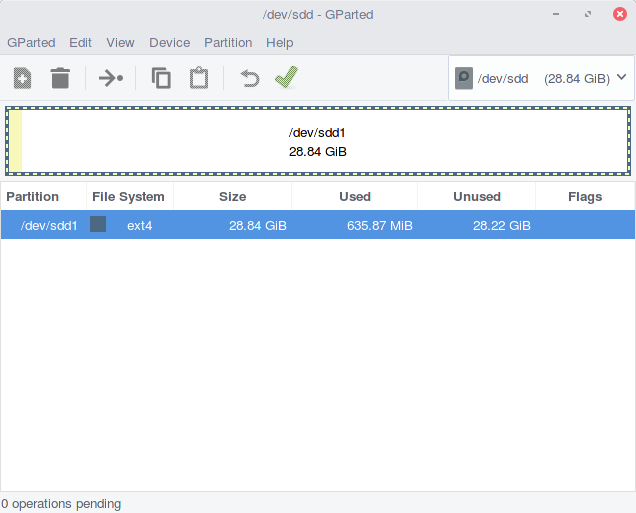
\includegraphics[width=0.45\textwidth]{img/luks/gparted1.png}
    }
    \hfill
    \subfloat[Redimensionnement de la partition principale]{%
      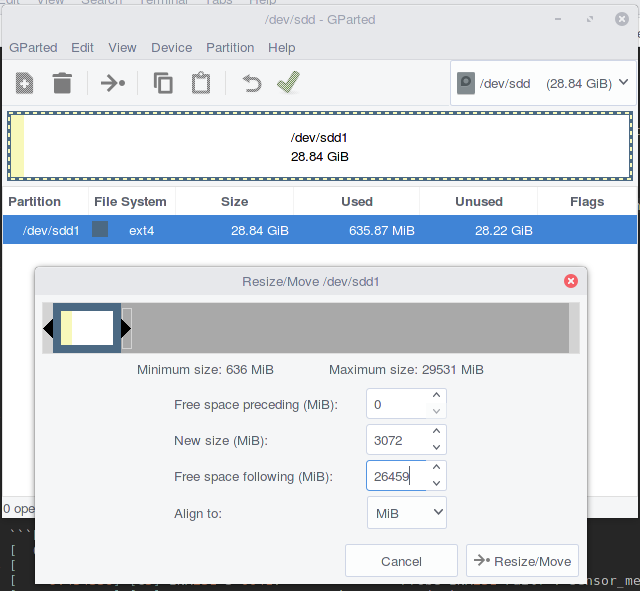
\includegraphics[width=0.45\textwidth]{img/luks/gparted2.png}
    }

    \subfloat[Création de la partition pour les données Docker]{%
      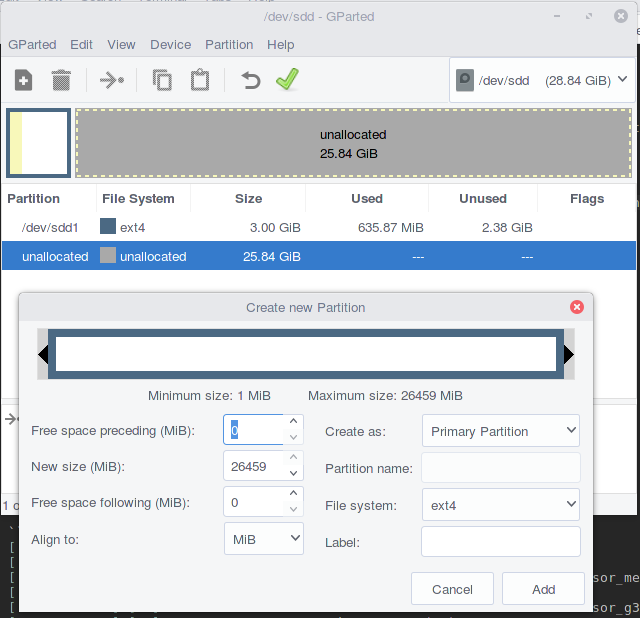
\includegraphics[width=0.45\textwidth]{img/luks/gparted3.png}
    }
    \hfill
    \subfloat[Confirmation]{%
      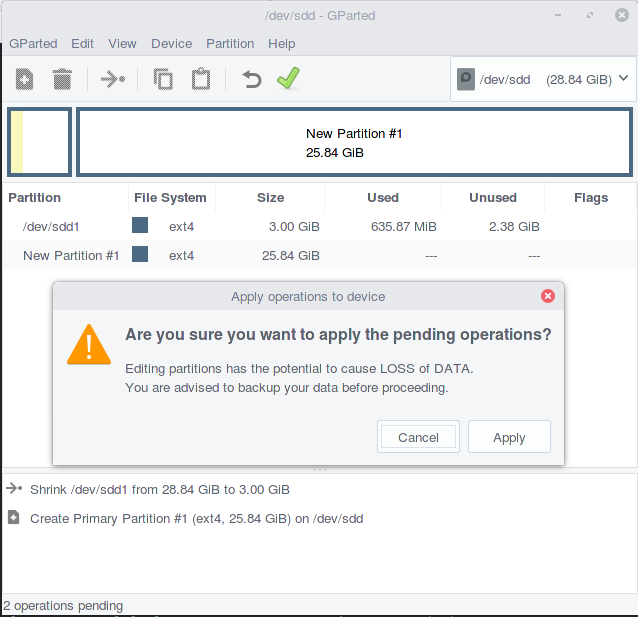
\includegraphics[width=0.45\textwidth]{img/luks/gparted4.png}
    }

     \subfloat[Partitionnement en cours...]{%
      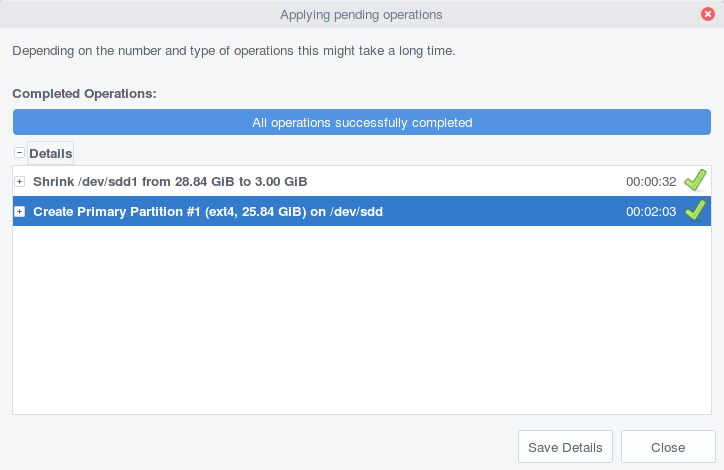
\includegraphics[width=0.45\textwidth]{img/luks/gparted5.png}
    }
    \hfill
    \subfloat[Situation finale - Deux partitions, la principale et celle pour Docker]{%
      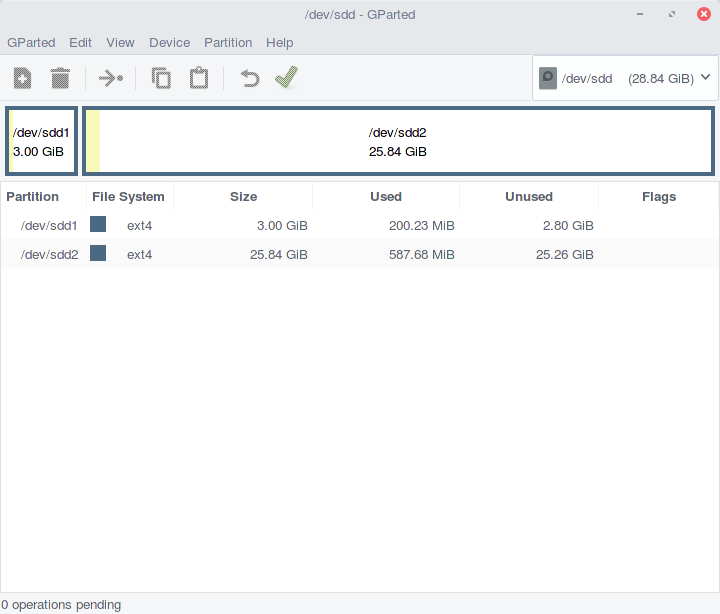
\includegraphics[width=0.45\textwidth]{img/luks/gparted6.png}
    }
    \caption{Redimensionnement de la partition principale}
\end{figure}

\subsection{Création d'une partition chiffrée}

Maintenant que la carte SD correctement partitionnée, il faut créer la partition chiffrée avec LUKS. Pour ce faire, Gnome Disks Utility est utilisé\footnote{Gnome Disk Utility : \url{https://doc.ubuntu-fr.org/gnome-disk-utility}}.

\begin{figure}[H]
    \subfloat[Sélection de la partition à chiffrer. Cliquer sur la roue crantée et sélectionner "Format Partition...".]{%
      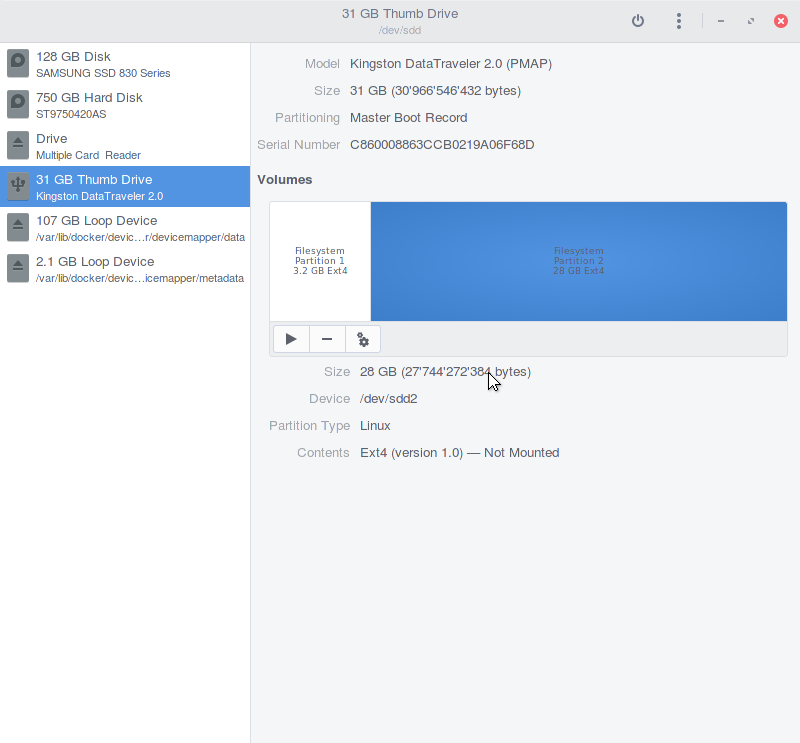
\includegraphics[width=0.45\textwidth]{img/luks/gnome-disks1.png}
    }
    \hfill
    \subfloat[Sélectionner "Encrypted, compatible with Linux systems (LUKS + ext4)" et saisir une passphrase (mot de passe)]{%
      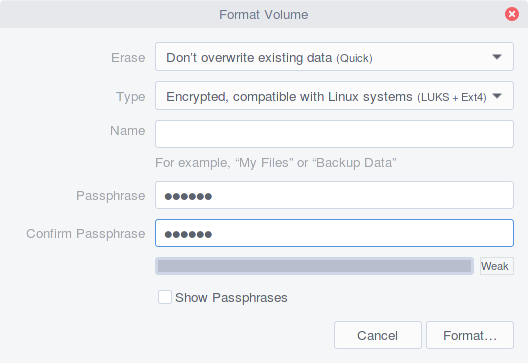
\includegraphics[width=0.45\textwidth]{img/luks/gnome-disks2.png}
    }

    \subfloat[La partition chiffrée est créée]{%
      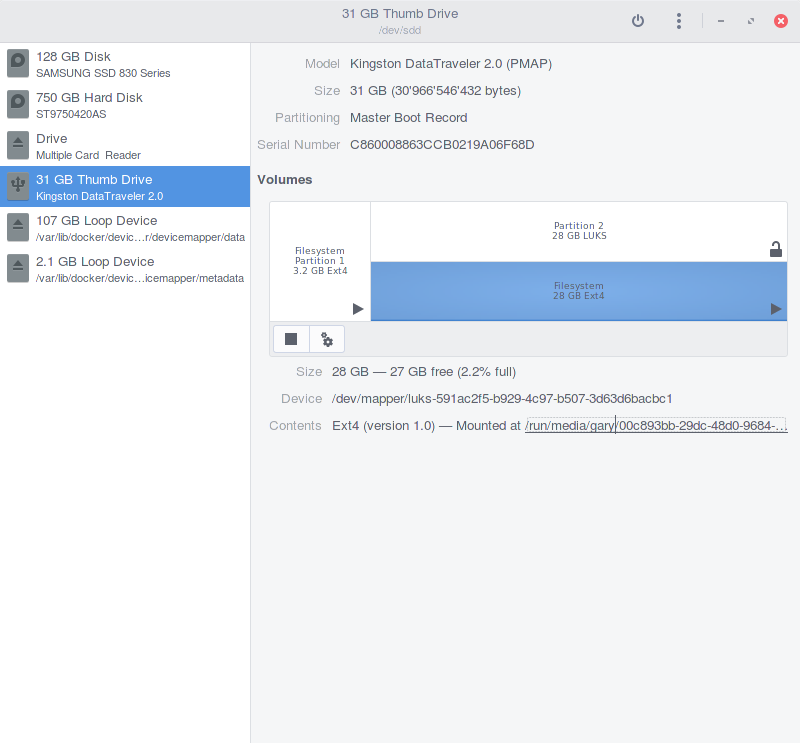
\includegraphics[width=0.45\textwidth]{img/luks/gnome-disks3.png}
    }
    \caption{Création de la partition chiffrée avec Gnome Disk Utility}
\end{figure}


\subsection{Montage manuel de la partition chiffrée}
Maintenant que la partition chiffrée a été créée, on peut replacer la carte SD dans la cible et la démarrer.

Pour monter manuellement la partition, il faut réaliser les commandes suivantes :
\begin{bashcode}
sudo mkdir /mnt/docker-data
sudo cryptsetup luksOpen /dev/mmcblk0p2 docker-data
sudo mount /dev/mapper/docker-data /mnt/docker-data/
\end{bashcode}

\code{/dev/mmcblk0p2} représente la partition chiffrée de la carte SD.

\subsection{Montage au boot de la partition chiffrée}
Monter manuellement la partition n'est pas une solution possible si l'on souhaite y mettre les données de Docker dessus. En effet, pour que Docker stocke ces données (rappel: les images et les containers) dans la partition chiffrée, il faut monter cette partition au démarrage de la cible et créer un \textit{bind mount} sur \code{/var/lib/docker}.


Avant d'effectuer le \textit{bind mount}, il faut faire en sorte de monter la partition chiffrée au boot.


Pour monter la partition chiffrée au démarrage du système, il faut ouvrir le fichier \code{/etc/crypttab} sur la cible, et ajouter la ligne suivante :
\begin{bashcode}
docker-data /dev/mmcblk0p2  none luks
\end{bashcode}

De manière similaire, il faut ajouter cette ligne dans le fichier \code{/etc/fstab} :
\begin{bashcode}
/dev/mapper/docker-data /mnt/docker-data ext4 rw 0 0
\end{bashcode}


\subsection{Preuve de bon fonctionnement du montage automatique}
Pour vérifier que tout ceci fonctionne bien, il suffit de redémarrer la cible et on devrait observer les lignes suivantes au boot :

\begin{bashcode}
[  OK  ] Found device /dev/mmcblk0p2.
         Starting Cryptography Setup for docker-data...
Please enter passphrase for disk docker-data on /mnt/docker-data! ******
[***   ] (1 of 2) A start job is running for...for docker-data (13s / no limit)[   22.871246] [c5] NET: Registered pr8
[**    ] (1 of 2) A start job is running for...for docker-data (13s / no limit)[   23.925487] [c6] bio: create slab <1
[  OK  ] Found device /dev/mapper/docker-data.
[  OK  ] Started Cryptography Setup for docker-data.
[  OK  ] Reached target Encrypted Volumes.
         Mounting /mnt/docker-data...
[   24.117386] [c5] EXT4-fs (dm-0): mounted filesystem with ordered data mode. Opts: (null)
[  OK  ] Mounted /mnt/docker-data.
\end{bashcode}

Le système va se bloquer pour que la saisie de la passphrase soit effectuée :
\begin{bashcode}
Please enter passphrase for disk docker-data on /mnt/docker-data! ******
\end{bashcode}

Une fois connecté, il est tout à fait possible de d'écrire des données sur la partition chiffrée :
\begin{bashcode}
echo "LUKS je suis ton père !" > /mnt/docker-data/starwars.txt
\end{bashcode}


\subsection{Binding des données de Docker sur la partition chiffrée}
Maintenant, on veut faire en sorte que les données de Docker soient dans cette partition chiffrée. Pour ce faire, on va effectuer un \textit{bind mount} entre un dossier dans la partition chiffrée et le dossier de Docker.

Un \textit{bind mount} n'est rien d'autre qu'un montage de dossier dans un autre dossier. On va donc monter \code{/mnt/docker-data/docker} dans \code{/var/lib/docker}. De cette manière, aucune configuration supplémentaire de Docker n'est nécessaire et ceci est donc complètement transparent pour lui. Cette opération est persistante après un redémarrage. Les \textit{bind mount} sont également utilisés comme redirection pour ne pas avoir de points de montage introuvables s'ils ont été déplacés.

\textbf{Attention : } Les opérations suivantes impliquent la perte de toutes les images et containers précédemment créés.

Création du dossier \code{docker} sur la partition chiffrée, à faire sur la cible :
\begin{bashcode}
sudo systemctl stop docker # on stoppe le service Docker avant tout
cd /mnt/docker-data
mkdir -p var/lib/docker
sudo rm -rf /var/lib/docker/ # supprime toutes les données de Docker !!!
sudo mkdir /var/lib/docker
\end{bashcode}

Sur la cible, on fait ensuite un \textit{bind mount} entre la partition chiffrée et le dossier Docker de base

\begin{bashcode}
sudo vim /etc/fstab

# dans ce fichier, on ajoute la ligne suivante
/mnt/docker-data/var/lib/docker /var/lib/docker none bind 0 0
\end{bashcode}

A la suite de ces modifications, le fichier /etc/fstab ressemble à ceci:
\begin{bashcode}
#
# /etc/fstab: static file system information
#
# <file system> <dir>   <type>  <options>       <dump>  <pass>
/dev/mapper/docker-data /mnt/docker-data ext4 rw 0 0
/mnt/docker-data/var/lib/docker /var/lib/docker none bind 0 0
\end{bashcode}


Désormais les données de Docker sont stockées sur une partition séparée et chiffrée. Pour prouver que c'est bien le cas, il suffit de relancer le benchmark de sécurité:

\begin{bashcode}
cd /home/alarm/docker/docker-bench-security
sudo bash docker-bench-security.sh

# la sortie indique:
[PASS] 1.1  - Create a separate partition for containers
\end{bashcode}


\subsection{Analyse de la solution proposée}
Stocker les données de Docker dans une partition chiffrée est une bonne initiative mais il faut garder à l'esprit les implications suivantes :
\begin{itemize}

\item La partition chiffrée est montée au boot. Ceci implique quand cas de reboot de la machine, il faut avoir un accès physique à celle-ci car le service ssh n'est pas encore lancé à ce moment là. En cas de dépannage à distance, il n'est pas donc possible de reboot la cible.
\item Les performances quand on utilise Docker devraient être diminuées dû au chiffrement
\item L'utilisation d'une partition séparée permet de réinstaller le système sans perdre les données liées à Docker et ses containers.
\item Le chiffrement des containers Docker apporte une plus value en terme de sécurité
\end{itemize}

\section{Conclusion sur la configuration du système d'exploitation hôte}
TODO dire ce qui s'est passé et ce qui serait bien de faire en plus (project nautilus), GRSecurity, SELinux, AppArmor.


\chapter{Création et utilisation des images Docker}\label{creation_utilisation_images_docker}
TODO : ce chapitre montre comment et pourquoi créer et utiliser des images Docker qui soient sécurisées et adaptées au monde de l'embarqué (taille principalement). Utilisation des hash cryptographiques pour l'OS utilisé et les versions des logiciels installés.
Montrer un cas pratique avec une image commune basée sur alpine linux dire ce que ca apporte de travailler ainsi et pourquoi il faut le faire.


\chapter{Utilisation des containers}\label{utilisation_containers}
TODO : parler de la philosophie des containers légers et éphémères, comment les exécuter de manière sûre et sécurisée, comment limiter le pouvoir des containers (conso ram, ddos, communication avec le monde extérieur ou entre containers, ...)

\begin{landscape}
\chapter{Déroulement du projet}


\section{Planning initial}
\begin{figure}[ht]
\centering
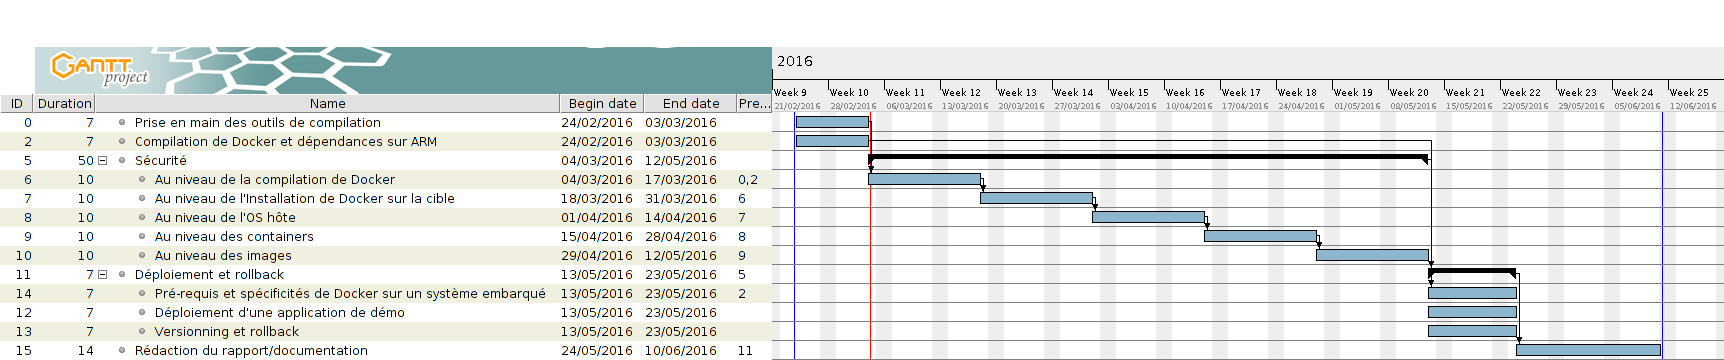
\includegraphics[height=4.7cm]{img/initial_planning.png}
\caption{Planning initial - 04.03.2016}
\end{figure}


\section{Planning final}
\begin{figure}[ht]
\centering
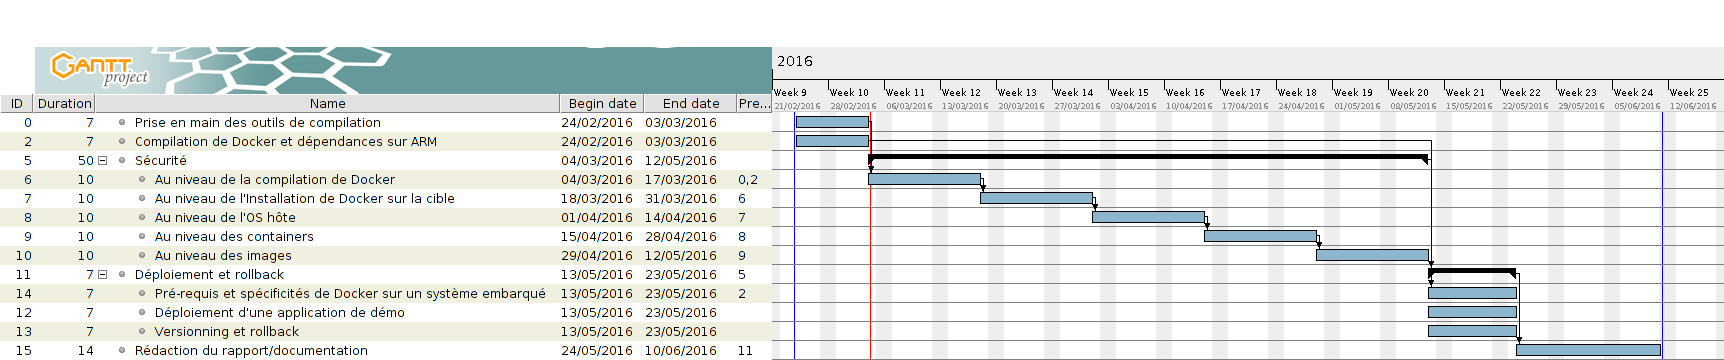
\includegraphics[draft,height=4.7cm]{img/initial_planning.png}
\caption{Planning final - TODO date}
\end{figure}

\end{landscape}
\chapter{Proposition d'améliorations vis à vis du travail précédent}
TODO: Pas prioritaire, a voir si on a le temps ! passer en revue et critique positivement le travail de Bachelor précédent. Dire que ce n'est pas une critique négative mais apporter un avis supplémentaire et plus récent (Docker évoluant beaucoup)

Arrivé en fin de projet, les rapports de M. Bassang ont été relus afin de voir, si avec le recul, il y avait de nouvelles choses à en tirer. Après cette lecture, il a été jugé intéressant de faire une critique positive sur le travail effectué et les recommandations données dans ces rapports. 

Le but ici est d'apporter un avis un peu moins informel, supplémentaire, complémentaire et plus récent sur l'utilisation de Docker en général.

Il faut insister sur le fait qu'il s'agit d'une critique positive qui a pour but d'améliorer le travail effectué. Avoir un feedback sur un projet est toujours bon à prendre.




\chapter{Conclusion}
TODO... ce qu'on voulait faire, ce qui a été fait, ce qu'il reste à faire/pourrait faire


% == Bibliography
\nocite{*} % cite all
\bibliographystyle{plain}
\bibliography{bibliography}

\begin{appendices}
\chapter{Installation de Archlinux ARM sur \odroid}\label{install_alarm_odroid}

\textbf{Remarque : }Ce guide requiert l'utilisation d'un ordinateur sous GNU/Linux.

Source : \url{https://archlinuxarm.org/platforms/armv7/samsung/odroid-xu3}

\section{Micro SD Card Creation}

Replace sdX in the following instructions with the device name for the SD card as it appears on your computer.

\begin{enumerate}

\item Zero the beginning of the SD card:

\begin{bashcode}
dd if=/dev/zero of=/dev/sdX bs=1M count=8
\end{bashcode}


\item Start fdisk to partition the SD card:

\begin{bashcode}
fdisk /dev/sdX
\end{bashcode}
 

\item At the fdisk prompt, create the new partitions:
	\begin{enumerate}[a.]
		        \item Type o. This will clear out any partitions on the drive.
		        \item Type p to list partitions. There should be no partitions left.
		        \item Type n, then p for primary, 1 for the first partition on the drive, and enter twice to accept the default starting and ending sectors.
		        \item Write the partition table and exit by typing w.
	\end{enumerate}
\item Create and mount the ext4 filesystem:

\begin{bashcode}
mkfs.ext4 /dev/sdX1
mkdir root
mount /dev/sdX1 root
\end{bashcode}


\item Download and extract the root filesystem (as root, not via sudo):

\begin{bashcode}
wget http://os.archlinuxarm.org/os/ArchLinuxARM-odroid-xu3-latest.tar.gz
bsdtar -xpf ArchLinuxARM-odroid-xu3-latest.tar.gz -C root
\end{bashcode}

\item Flash the bootloader files:

\begin{bashcode}
cd root/boot
sh sd_fusing.sh /dev/sdX
cd ../..
\end{bashcode}


\item    (Optional) Set the MAC address for the onboard ethernet controller:
    \begin{enumerate}[a.]
        \item Open the file root/boot/boot.ini with a text editor.
        \item Change the MAC address being set by the setenv macaddr command to the desired address.
        \item Save and close the file.
    \end{enumerate}

\item    Unmount the partition:

    umount root

\item    Set the boot switches on the ODROID-XU3 board to boot from SD:
    \begin{enumerate}[a.]
        \item With the board oriented so you can read the ODROID-XU3 on the silkscreen, locate the two tiny switches to the left of the ethernet jack.
        \item The first switch (left) should be in the off position, which is down.
        \item The second switch (right) should be in the on position, which is up.
    \end{enumerate}
    
\item    Insert the micro SD card into the XU3, connect ethernet, and apply 5V power.
\item    Use the serial console (with a null-modem adapter if needed) or SSH to the IP address given to the board by your router.
    \begin{itemize}
        \item Login as the default user alarm with the password alarm.
        \item The default root password is root.
    \end{itemize}

\end{enumerate}

\section{eMMC Module Creation}

\begin{enumerate}
\item    Attach the eMMC module to the micro SD adapter, and plug that into your computer.

\item    Follow the above steps to install Arch Linux ARM, and boot the board with the eMMC still attached to micro SD adapter, plugged into the SD slot in the board.

\item    Re-flash the bootloader to the protected boot area of the eMMC module:
\begin{bashcode}
cd /boot
./sd_fusing.sh /dev/mmcblk0
\end{bashcode}

\item    Power off the board:
\begin{bashcode}
poweroff
\end{bashcode}

\item    Remove the micro SD adapter, and detach the eMMC module.

\item    Set the boot switches on the ODROID-XU3 board to boot from eMMC:
    \begin{enumerate}[a.]
        \item With the board oriented so you can read the ODROID-XU3 on the silkscreen, locate the two tiny switches to the left of the ethernet jack.
        \item The first switch (left) should be in the on position, which is up.
        \item The second switch (right) should be in the on position, which is up.
    \end{enumerate}
    
\item    Connect the eMMC module to the XU3, ensuring you hear a click when doing so, connect ethernet, and apply 5V power.

\item    Use the serial console (with a null-modem adapter if needed) or SSH to the IP address given to the board by your router.
    \begin{itemize}
        \item Login as the default user alarm with the password alarm.
        \item The default root password is root.
    \end{itemize}

\end{enumerate}

\end{appendices}

\end{document}
